% Exact source-layer transcription of Xi Yin, Physics 253a,
% original note pp. 10--29; combined source PDF physical pp. 21--40.
% Combined source PDF:
%   /Users/wlancer/Desktop/IAS/phy/qft/qft_253abc_book.pdf
% Source SHA-256:
%   9e5e4d241fffffa56c1c3df6dce4b83178f75787dd5d794a18c5d0c087769f21
%
% This is a literal note-layer capture. Source order, line fragments,
% punctuation, colors, arrows, braces, corrections, questions, and diagrams
% are retained. No source notation is silently normalized.
%
% Open source readings are tied to:
%   work/253a-ch02/ambiguities.md
%
% Compilation requirements for reconstructed diagrams:
%   xcolor, tikz, tikz libraries arrows.meta, positioning,
%   decorations.pathmorphing.

\providecommand{\YinPageBoundary}[2]{%
  \clearpage
  \noindent\textsf{[Original Physics 253a note p.~#1; combined PDF physical p.~#2]}%
  \par\medskip
}
\providecommand{\YinLine}[1]{\noindent #1\par}
\providecommand{\YinIndent}[1]{\noindent\hspace*{2em}#1\par}
\providecommand{\YinBullet}[1]{\noindent\hspace*{1em}$\bullet$\hspace{0.7em}#1\par}
\providecommand{\YinDash}[1]{\noindent\hspace*{1em}--\hspace{0.7em}#1\par}
\providecommand{\YinBlue}[1]{{\color[rgb]{0.00,0.34,0.92}#1}}
\providecommand{\YinLightBlue}[1]{{\color[rgb]{0.47,0.67,0.82}#1}}
\providecommand{\YinPurple}[1]{{\color[rgb]{0.61,0.16,0.88}#1}}
\providecommand{\YinGray}[1]{{\color[rgb]{0.58,0.58,0.58}#1}}
\providecommand{\YinGreen}[1]{{\color[rgb]{0.00,0.52,0.22}#1}}
\providecommand{\YinRed}[1]{{\color[rgb]{0.95,0.18,0.10}#1}}
\providecommand{\YinMagenta}[1]{{\color[rgb]{0.75,0.00,0.55}#1}}
\providecommand{\YinOrange}[1]{{\color[rgb]{0.95,0.43,0.00}#1}}
\providecommand{\ket}[1]{\lvert #1\rangle}
\providecommand{\bra}[1]{\langle #1\rvert}
\providecommand{\braket}[2]{\langle #1\mid #2\rangle}

% ---------------------------------------------------------------------------
\YinPageBoundary{10}{21}

\YinLine{\underline{Lagrangian formalism}}
\YinLine{Recall in classical mechanics:}

% The source is a two-column comparison. The blue U-shaped connector has
% arrowheads at both rising ends and the words related by below it.
\begin{center}
\begin{tikzpicture}[
  x=1cm,y=1cm,
  every node/.style={font=\small},
  >=Stealth
]
  \node (lag) at (-4.1,0) {Lagrangian};
  \node (vs) at (0,0) {vs};
  \node (ham) at (4.1,0) {Hamiltonian};

  \node[anchor=north west,align=left] at (-6.1,-0.55) {%
    \text{\textquotedblleft state\textquotedblright}\hspace{1.6em} $q,\dot q$};
  \node[anchor=north west,align=left] at (1.9,-0.55) {%
    $q,p.$};

  \node[anchor=north west,align=left] at (-6.1,-1.45) {%
    EOM\hspace{2.2em} extremize};
  \node[anchor=north west,align=left] at (1.9,-1.45) {%
    $\dot f=\{H,f\}_{\mathrm{Poisson}}$};

  \node[anchor=north west,align=left] at (-2.1,-2.35) {%
    $S=\displaystyle\int dt\,L(q,\dot q)$};
  \node[anchor=north west,align=left,text=gray] at (1.85,-2.35) {%
    \begin{gathered}
      \text{\YinGray{e.g.}}\quad
      \dot q=\dfrac{\partial H}{\partial p},\\[3pt]
      \dot p=-\dfrac{\partial H}{\partial q}.
    \end{gathered}};

  \draw[blue,->,line width=0.85pt]
    (-3.2,-3.1) .. controls (-3.2,-4.15) and (3.2,-4.15) .. (3.2,-3.1);
  \draw[blue,->,line width=0.85pt]
    (3.2,-3.1) .. controls (3.2,-4.15) and (-3.2,-4.15) .. (-3.2,-3.1);
  \node[blue] at (0,-4.28) {related by};
  \node[blue,align=center] at (0,-5.05) {%
    $\displaystyle H(p,q)=
      \left.p\dot q-L(q,\dot q)\right|_{\frac{\partial L}{\partial\dot q}=p}$};

  \draw[blue,dashed,line width=0.7pt] (0,-5.45) -- (0,-10.8);
  \node[anchor=west] at (-6.1,-6.05) {QM:};
  \node at (-3.9,-6.05) {Hamiltonian};
  \node at (0,-6.05) {vs};
  \node at (3.8,-6.05) {Lagrangian};

  \node[anchor=north west,align=left] at (-6.1,-6.55) {%
    State\hspace{1.25em} $|\psi\rangle\in\mathcal H$\\[5pt]
    \hspace*{1.5em}$H(p,q)\leadsto\hat H$};
  \node[anchor=north west] at (1.9,-6.55) {%
    $\displaystyle S=\int dt\,L(q,\dot q)$};
\end{tikzpicture}
\end{center}

% PAGE-TRANSITION: physical p. 21 closes the classical comparison and begins
% the quantum-mechanics comparison at the lower margin.

% ---------------------------------------------------------------------------
\YinPageBoundary{11}{22}

% The upper half is a two-column comparison separated by a blue dashed line.
\begin{center}
\begin{tikzpicture}[
  every node/.style={font=\small},
  >=Stealth
]
  \node[anchor=north west,align=left] at (-7.2,0) {%
    time\\[-1pt] evolution};
  \draw[blue,dashed,line width=0.75pt] (0.0,0.2) -- (0.0,-5.6);

  \node[anchor=north west,align=left] at (-5.95,0) {%
    Schr\"odinger:\\[5pt]
    $\displaystyle|\psi\rangle\mapsto U(t)|\psi\rangle,$\\[7pt]
    $\displaystyle U(t)=e^{-\frac{i}{\hbar}\hat Ht}$\\[10pt]
    Heisenberg:\\[5pt]
    $\displaystyle O\mapsto
      \underbrace{(U(t))^{-1}OU(t)}_{
        \YinBlue{\substack{\text{|||}\\[-3pt]O(t)}}}.$\\[8pt]
    $\displaystyle\dot O(t)=\frac{i}{\hbar}[\hat H,O(t)]$};

  \node[anchor=north west,align=left] at (0.55,0) {%
    $\displaystyle\langle q_f|U(T)|q_i\rangle$\\[7pt]
    $\displaystyle=
      \int_{q(0)=q_i}^{q(T)=q_f}[Dq]\,
      e^{\frac{i}{\hbar}S}$};
\end{tikzpicture}
\end{center}

% AMBIGUITY P22-A1: three short blue marks above O(t) under the Heisenberg
% underbrace have no settled symbolic reading. See
% work/253a-ch02/ambiguities.md.

\begin{center}
\begin{tikzpicture}[baseline,>=Stealth]
  \node (measure) {$[Dq]$};
  \draw[magenta,line width=0.8pt,decorate,
    decoration={snake,amplitude=0.30mm,segment length=1.8mm}]
    (measure.south west) -- (measure.south east);
  \draw[magenta,->,line width=0.8pt]
    (measure.north) to[out=100,in=-90] (0.3,1.0);
  \node[magenta,anchor=west] at (0.38,1.0) {what is this ?};
\end{tikzpicture}
\end{center}

\YinBullet{Much of the subtleties with the Lagrangian
  formulation of QM have to do with the
  path integral measure [Dq].}
\YinLine{Let us revisit its derivation:}
\YinLine{Consider the time evolution by T}
\YinIndent{in N steps,}

\begin{center}
\begin{tikzpicture}[x=1cm,y=1cm,>=Stealth,every node/.style={font=\small}]
  \draw[line width=0.7pt] (-5,0) -- (5,0);
  \foreach \x/\lab in {-5/$q_i$,-3.35/$q_1$,-1.70/$q_2$,
                         0/$q_3$,1.65/$\cdots$,3.25/$q_{N-1}$,5/$q_f$} {
    \draw[line width=0.7pt] (\x,-0.10) -- (\x,0.10);
    \node[above=2pt] at (\x,0.10) {\lab};
  }
  \node[below=5pt] at (-5,0) {0};
  \node[below=5pt] at (5,0) {T};
  \draw[blue,line width=0.75pt,decorate,
    decoration={brace,amplitude=4pt,mirror}]
    (-5,-0.28) -- (-3.35,-0.28);
  \node[blue,below=9pt] at (-4.18,-0.28) {T/N};
\end{tikzpicture}
\end{center}

% PAGE-TRANSITION: the time-slicing diagram reaches the lower margin as an
% open derivation boundary. The next page inserts position and momentum
% resolutions and expands the short-time Hamiltonian factors.

% ---------------------------------------------------------------------------
\YinPageBoundary{12}{23}

\[
 \langle q_f\mid U(T)\mid q_i\rangle
\]
\[
\begin{aligned}
={}&\int d^Dq_1\,\cdots\,d^Dq_{N-1}\,
 \langle q_f\mid e^{-\frac{i}{\hbar}\hat H\,\cdot\,\frac{T}{N}}
       \mid q_{N-1}\rangle
 \,\cdots\,
 \langle q_1\mid e^{-\frac{i}{\hbar}\hat H\,\cdot\,\frac{T}{N}}
       \mid q_i\rangle
\end{aligned}
\]
\YinLine{\YinBlue{[ denote $q_f\equiv q_N,\qquad q_i\equiv q_0$ ]}}
\[
\begin{aligned}
={}&\int\prod_{n=1}^{N-1}d^Dq_n\;\cdot\;
 \prod_{n=0}^{N-1}
 \langle q_{n+1}\mid
 e^{-\frac{i}{\hbar}\hat H\,\cdot\,\frac{T}{N}}
 \mid q_n\rangle .
\end{aligned}
\]

% The long blue curved arrow selects one short-time factor and inserts the
% momentum resolution shown below.
\begin{center}
\begin{tikzpicture}[baseline,>=Stealth]
  \node (from) at (-2.2,0)
    {$\prod\langle q_{n+1}\mid e^{-\frac{i}{\hbar}\hat H\frac{T}{N}}
       \mid q_n\rangle$};
  \node[blue,anchor=west] (to) at (1.2,-0.55)
    {$\displaystyle\int\frac{d^Dp_n}{(2\pi\hbar)^D}
      \langle q_{n+1}\mid p_n\rangle
      \langle p_n\mid e^{-\frac{i}{\hbar}\hat H\frac{T}{N}}
      \mid q_n\rangle$};
  \draw[blue,->,line width=0.8pt]
    (from.south east) to[out=-25,in=145] (to.north west);
\end{tikzpicture}
\end{center}

\[
\YinBlue{%
\begin{aligned}
 &\underbrace{\langle q_{n+1}\mid p_n\rangle}_{\text{\scriptsize two short strokes}}\\[-2pt]
 &\hspace{4em}
 =e^{\frac{i}{\hbar}p_n\cdot q_{n+1}}
\end{aligned}}
\qquad
\YinBlue{%
\underbrace{\left\langle p_n\middle|
 e^{-\frac{i}{\hbar}\hat H\,\frac{T}{N}}\middle|q_n\right\rangle}_{
 \YinBlue{\scriptstyle\text{\raisebox{1pt}{\(\approx\!\approx\)}}}}
 \approx
 e^{-\frac{i}{\hbar}H(q_n,p_n)\frac{T}{N}}
 e^{-\frac{i}{\hbar}p_n\cdot q_n}}
\]

\YinLine{\YinMagenta{classical Hamiltonian}
  \hspace{1em}\YinMagenta{$\uparrow$}\hspace{1em}
  $H(q_n,p_n)$}
\[
\begin{aligned}
={}&\int\prod_{n=1}^{N-1}d^Dq_n
 \prod_{n=0}^{N-1}\frac{d^Dp_n}{(2\pi\hbar)^D}\\[-2pt]
&\quad\cdot\exp\left\{
 \frac{i}{\hbar}\sum_{n=0}^{N-1}
 \left[
 p_n\cdot(q_{n+1}-q_n)
 -H(q_n,p_n)\frac{T}{N}
 +O\left(\hbar,\left(\frac{T}{N}\right)^2\right)
 \right]\right\}.
\end{aligned}
\]

% AMBIGUITY P23-A1: the first blue underbrace has a small mark resembling
% 11 and the second has a double-wavy mark resembling an approximation sign
% or an unreadable label. See work/253a-ch02/ambiguities.md.
% AMBIGUITY P23-A2: the source uses the visible O-term glyph captured as
% O(hbar,(T/N)^2). No higher-layer normalization is made here.

% PAGE-TRANSITION: physical p. 23 closes with the finite-N phase-space
% expression and its O(hbar,(T/N)^2)-type remainder. Physical p. 24 takes
% the formal N to infinity limit.

% ---------------------------------------------------------------------------
\YinPageBoundary{13}{24}

\YinLine{\text{formally, in }N\to\infty\
  \text{\textquotedblleft limit\textquotedblright}}
\[
\begin{aligned}
={}&\int\mathcal Dq\,\mathcal Dp\;
 e^{\frac{i}{\hbar}\int_0^Tdt\,(p\cdot\dot q-H(q,p))}.
\end{aligned}
\]
\begin{center}
\begin{tikzpicture}[baseline,>=Stealth,every node/.style={font=\small}]
  \node (measure) {$\mathcal Dq\,\mathcal Dp$};
  \node[blue,align=left,anchor=west] (reg) at (1.4,0.05) {%
    defined via\\[-1pt] regularization\\[-1pt] e.g. discretizing time};
  \draw[blue,->,line width=0.75pt]
    (measure.south) to[out=-80,in=170] (reg.west);
  \node (h) at (0,-1.0) {$H(q,p)$};
  \node[blue,align=left,anchor=west] (amb) at (1.4,-1.0) {%
    Contains $O(\hbar)$ ambiguities\\[-1pt]
    -- \textquotedblleft counter terms\textquotedblright\\[-1pt]
    -- these ambiguities\\[-1pt]
    \hspace*{1em}are tied to the scheme\\[-1pt]
    \hspace*{1em}of regularization.};
  \draw[blue,->,line width=0.75pt]
    (h.east) to[out=0,in=180] (amb.west);
\end{tikzpicture}
\end{center}

% AMBIGUITY P24-A1: the handwritten O glyph resembles a small t with an
% h-like component. The exact-layer capture uses O(hbar). See
% work/253a-ch02/ambiguities.md.
\YinLine{\YinGray{An example of alternative time-lattice regularization:}}
\[
\YinGray{%
\int_0^Tdt\;p\cdot\dot q
\longrightarrow
\sum_{n=0}^{N-1}p_n\cdot(q_{n+1}-q_n)}
\]
\[
\YinGray{\text{versus}\qquad
\sum_{n=0}^{N-1}p_{n+1}\cdot(q_{n+1}-q_n)}
\]
\YinLine{\YinGray{The exact representation of the time evolution is}}
\[
\YinGray{%
\cdots\,\langle q_{n+1}\mid p_n\rangle
\langle p_n\mid e^{-\frac{i}{\hbar}\hat H\,\frac{T}{N}}
\mid q_n\rangle\,\cdots}
\]
\YinLine{\YinGray{in the former case, and}}
\[
\YinGray{%
\langle p_n\mid\hat H\mid q_n\rangle
=H(p_n,q_n)\langle p_n\mid q_n\rangle}
\]
\[
\YinBlue{%
\cdots\,\langle p_{n+1}\mid q_n\rangle
\langle q_n\mid e^{-\frac{i}{\hbar}\hat H\,\frac{T}{N}}
\mid p_n\rangle\,\cdots}
\]
\YinLine{\YinBlue{in the latter case}}
\[
\YinBlue{%
\langle q_n\mid\hat H\mid p_n\rangle
=H'(p_n,q_n)\langle q_n\mid p_n\rangle}
\]
\YinLine{%
  \YinPurple{$H(p_n,q_n)$}\ \text{and}\
  \YinBlue{$H'(p_n,q_n)$}\ \text{can differ at order }O(\hbar).}

% AMBIGUITY P24-A2: preserve H(q_n,p_n) in the finite-N exponent on p. 23,
% H(p_n,q_n) in the purple relation here, and H'(p_n,q_n) in the blue
% relation. See work/253a-ch02/ambiguities.md.
% PAGE-TRANSITION: physical p. 24 hands off the regularization discussion
% to the Gaussian momentum-integration case beginning on physical p. 25.

% ---------------------------------------------------------------------------
\YinPageBoundary{14}{25}

\YinLine{If $H(q,p)$ is quadratic in $p$.}
\YinLine{\YinGray{e.g.}\quad
  $H(q,p)=\dfrac{p^2}{2m}+V(q)$,}
\YinLine{we can integrate out $P(t)$ as Gaussian,}
\YinLine{leaving}
\[
\int[D\xi]\,
 e^{\frac{i}{\hbar}\int_0^Tdt\,(p\dot\xi-H)}
\bigg|_{\dot\xi=\frac{\partial H}{\partial p}}
\]
\begin{center}
\begin{tikzpicture}[baseline,>=Stealth,every node/.style={font=\small}]
  \node (measure) {$[D\xi]$};
  \node[blue,align=left,anchor=west] (det) at (1.4,0) {%
    absorbs Gaussian\\[-1pt] determinant of $P(t)$};
  \draw[blue,->,line width=0.75pt]
    (det.west) to[out=180,in=0] (measure.east);
\end{tikzpicture}
\end{center}
\begin{center}
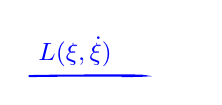
\begin{tikzpicture}[baseline,every node/.style={font=\small}]
  \node[blue] (laglabel) {$L(\xi,\dot\xi)$};
  \draw[blue,line width=0.75pt]
    (laglabel.south west) .. controls (-0.2,-0.3) and (1.5,-0.3) ..
    (laglabel.south east);
\end{tikzpicture}
\end{center}
\YinLine{\YinGray{More generally, Lagrangian in generalized coordinates}}
\YinLine{\YinGray{typically takes the form}}
\[
\YinGray{%
L=\frac{1}{2}G_{\alpha\beta}(\xi)\dot\xi^\alpha\dot\xi^\beta-V(\xi)}
\qquad
\YinGray{\left[\begin{array}{l}
\text{e.g. rotating}\\[-1pt]
\text{3D rigid body}
\end{array}\right]}
\]
\[
\YinGray{%
\Longleftrightarrow\quad
H=\frac{1}{2}\bigl(G^{-1}(\xi)\bigr)^{\alpha\beta}p_\alpha p_\beta
  +V(\xi)+\YinLightBlue{O(\hbar)}}
\]
\YinLine{\YinGray{Path integral}}
\[
\YinGray{%
\int\mathcal Dp\,\mathcal D\xi\,
e^{\frac{i}{\hbar}\int dt\,
(p_\alpha\dot\xi^\alpha-H(p,\xi))}
=
\int[D\xi]\,
e^{\frac{i}{\hbar}\int dt\,L(\xi,\dot\xi)}}
\]
\[
\YinGray{%
[D\xi]\;\leadsto\;
\prod_{n=1}^{\widetilde N}
\frac{d\xi_n^\alpha}
{\sqrt{2\pi i\hbar\,\frac{T}{N}}}
\sqrt{\det G_{\alpha\beta}(\xi_n)}\, .}
\]

% AMBIGUITY P25-A1: the source prose and determinant note visibly use P(t),
% while the phase-space equations use p. Preserve the visible P(t). See
% work/253a-ch02/ambiguities.md.
% AMBIGUITY P25-A2: the handwritten Dp Dxi measures do not settle
% calligraphic status or differential subscripts. The source-layer surrogate
% above preserves the visible measure variables.
% AMBIGUITY P25-A3: xi is retained as the generalized-coordinate glyph.
% AMBIGUITY P25-A4: the pale-blue correction is captured as +O(hbar).
% AMBIGUITY P25-A5: the product upper limit has a tilde, while the square
% root visibly contains T/N. Both forms are kept.
% AMBIGUITY P25-A6: the evaluation bar is placed after the full displayed
% phase-space factor as visually reported. See work/253a-ch02/ambiguities.md.
% PAGE-TRANSITION: physical p. 25 ends after the discretized measure.
% Physical p. 26 begins a new correlation-function bullet.

% ---------------------------------------------------------------------------
\YinPageBoundary{15}{26}

% The leading dot is a source mark at the left margin.
\YinLine{. Consider correlation function in}
\YinIndent{ground state $|0\rangle$, \quad e.g.}
\[
G(t)\equiv\langle 0|\hat q_{\beta}(t)\,\hat q_{\beta}(0)|0\rangle
\]
\[
=\sum_n\langle 0|\hat q_{\beta}(t)|n\rangle
  \langle n|\hat q_{\beta}(0)|0\rangle
\]
\begin{center}
\begin{tikzpicture}[baseline,>=Stealth,every node/.style={font=\small}]
  \node (state) {$|n\rangle$};
  \draw[blue,line width=0.75pt,decorate,
    decoration={snake,amplitude=0.28mm,segment length=1.8mm}]
    (state.south west) -- (state.south east);
  \node[blue,anchor=west] (basis) at (0.85,0.15)
    {a basis of $\hat H$ - eigenstates};
  \draw[blue,->,line width=0.75pt]
    (state.north east) to[out=45,in=180] (basis.west);
\end{tikzpicture}
\end{center}
\[
\YinBlue{\hat H|n\rangle=E_n|n\rangle.}
\]
\[
\begin{aligned}
=\sum_n\,
\langle 0|e^{\YinBlue{\frac{i}{\hbar}}\hat Ht}
\hat q_{\beta}(0)e^{-\YinBlue{\frac{i}{\hbar}}\hat Ht}|n\rangle
\langle n|\hat q_{\beta}(0)|0\rangle
\end{aligned}
\]
\[
\begin{aligned}
=\sum_n\,
\langle 0|\hat q_{\beta}(0)|n\rangle
\langle n|\hat q_{\beta}(0)|0\rangle\,\cdot\,
e^{-\frac{i}{\hbar}(E_n-E_0)t}.
\end{aligned}
\]
\[
\underbrace{%
\langle 0|\hat q_{\beta}(0)|n\rangle
\langle n|\hat q_{\beta}(0)|0\rangle%
}_{\YinBlue{\substack{\text{\scriptsize |||}\\[-2pt]\beta_n,\ \text{some number}}}}
\]
\YinLine{As $E_n-E_0>0$, can analytically continue}
\YinLine{$G(t)$ as a function of complex $t$,}
\YinLine{provided $\operatorname{Im}t<0$. So that $\sum_n$ converges.}
\YinLine{\YinGray{[Paley-Wiener theorem]}}

% AMBIGUITY P26-A1: the blue coefficient label is captured as beta_n, with
% a possible cursive g_n reading for its first glyph. See
% work/253a-ch02/ambiguities.md.
% AMBIGUITY P26-A2: blue accents on the i/hbar factors are retained as
% source annotations; their editing chronology is unresolved.
% AMBIGUITY P26-A3: the leading margin dot before Consider is preserved as
% a source mark.
% PAGE-TRANSITION: physical p. 26 ends with the strict lower-half-plane
% convergence statement and the gray Paley-Wiener cue. Physical p. 27
% begins with t=-i tau and the quoted Wick rotation label.

% ---------------------------------------------------------------------------
\YinPageBoundary{16}{27}

\YinLine{e.g. \quad $t=-i\tau,\quad\tau\in\mathbb R_+$}
\YinLine{\text{\textquotedblleft Wick rotation\textquotedblright}}
\[
\langle 0|\hat q(t)\hat q(0)|0\rangle
=\sum_n
\langle 0|\hat q(0)|n\rangle
\langle n|\hat q(0)|0\rangle
\cdot e^{-\YinBlue{\frac{1}{\hbar}}(E_n-E_0)\tau}.
\]
\YinLine{Assuming a gap $\bar E_1-\bar E_0>0$, \quad can replace}
\YinLine{$|0\rangle$ \quad by\quad
  $\displaystyle\lim_{T\to\infty}
  e^{-\YinBlue{\frac{1}{\hbar}}(\hat H-E_0)T}|\psi\rangle,$}
\YinLine{up to overall normalization,}
\YinLine{for any generic state $|\psi\rangle$.}
\YinLine{\YinGray{(that has nonzero overlap with $|0\rangle$)}}
\[
\langle 0|\hat q(t)\hat q(0)|0\rangle
=\lim_{T\to\infty}
\frac{%
\langle\psi|
\underbrace{e^{-\YinBlue{\frac{1}{\hbar}}\hat H T}}_{\YinPurple{\text{\scriptsize left brace}}}
\hat q(t)\hat q(0)
\underbrace{e^{-\YinBlue{\frac{1}{\hbar}}\hat H T}}_{\YinBlue{\text{\scriptsize right brace}}}
|\psi\rangle}{%
\langle\psi|e^{-\YinBlue{\frac{2}{\hbar}}\hat H T}|\psi\rangle}.
\]
\YinLine{\YinRed{$\downarrow$ to $\hat q(t)$}\hspace{3em}
  \YinOrange{$\downarrow$ to $\hat q(0)$}}

\begin{center}
\begin{tikzpicture}[x=1cm,y=1cm,>=Stealth,every node/.style={font=\small}]
  \draw[->,line width=0.75pt] (-2.8,0) -- (3.8,0)
    node[right] {Re $t$};
  \draw[->,line width=0.75pt] (-2.0,-1.2) -- (-2.0,4.1)
    node[above] {-Im $t$};
  \draw[magenta,line width=1.1pt] (-2.0,0) -- (-2.0,3.15);
  \draw[magenta,->,line width=0.95pt] (-2.0,2.2) -- (-2.0,2.8);
  \draw[blue,line width=1.0pt] (-2.0,-1.0) -- (-2.0,0.25);
  \draw[blue,->,line width=0.9pt] (-2.0,-0.55) -- (-2.0,-0.05);
  \draw[green!55!black,line width=1.0pt]
    (-2.0,3.15) .. controls (-0.6,3.1) and (1.5,2.6) .. (2.7,1.0);
  \draw[green!55!black,line width=1.0pt]
    (-2.0,0.25) .. controls (-0.8,0.45) and (1.4,1.5) .. (2.7,1.0);
  \draw[green!55!black,->,line width=0.85pt]
    (1.5,0.95) -- (2.0,1.0);
  \fill[orange] (-2.0,0.25) circle (2.6pt);
  \fill[red] (2.7,1.0) circle (2.8pt);
\end{tikzpicture}
\end{center}

% AMBIGUITY P27-A1: the gap accents are horizontal bars, captured as
% bar E_1 minus bar E_0. The p. 27 contour has two green traces; only the
% lower one has a separately visible rightward arrow.
% PAGE-TRANSITION: physical p. 27 closes with the complex-t contour sketch.
% Physical p. 28 begins with Alternatively, and a straight Euclidean-time
% representation.

% ---------------------------------------------------------------------------
\YinPageBoundary{17}{28}

\YinLine{Alternatively,}
\[
G(t=-i\tau)
=\langle 0|e^{\YinBlue{\frac{1}{\hbar}}H\tau}
\hat q(0)e^{-\YinBlue{\frac{1}{\hbar}}H\tau}
\hat q(0)|0\rangle.
\]
\[
\begin{aligned}
G(t=-i\tau)
={}&\lim_{T\to\infty}
\frac{%
\langle\psi|
e^{-\YinBlue{\frac{1}{\hbar}}H(T-\tau)}
\hat q(0)
e^{-\YinBlue{\frac{1}{\hbar}}H\tau}
q(0)
e^{-\YinBlue{\frac{1}{\hbar}}HT}
|\psi\rangle}{%
\langle\psi|e^{-\YinBlue{\frac{2}{\hbar}}HT}|\psi\rangle}.
\end{aligned}
\]
\YinLine{\YinRed{$\downarrow$ to the first insertion}
  \hspace{3em}\YinOrange{$\downarrow$ to the second insertion}}

\begin{center}
\begin{tikzpicture}[x=1cm,y=1cm,>=Stealth,every node/.style={font=\small}]
  \draw[blue,line width=1.0pt] (-4.4,0) -- (1.7,0);
  \draw[black,->,line width=0.75pt] (1.7,0) -- (4.0,0)
    node[right] {-Im $t$};
  \draw[blue,line width=0.9pt] (-4.4,-0.16) -- (-4.4,0.16);
  \draw[blue,line width=0.9pt] (1.7,-0.16) -- (1.7,0.16);
  \fill[orange] (-1.9,0) circle (2.6pt);
  \fill[red] (-0.05,0) circle (2.6pt);
  \node[blue,below=3pt] at (-4.4,0) {-T};
  \node[orange,below=3pt] at (-1.9,0) {0};
  \node[red,below=3pt] at (-0.05,0) {$\tau$};
  \node[blue,below=3pt] at (1.7,0) {T};
\end{tikzpicture}
\end{center}

\YinLine{From path integral:}
\[
\langle 0|\hat q(t)\hat q(0)|0\rangle
=\lim_{\substack{\operatorname{Im}t_f\to-\infty\\
                  \operatorname{Im}t_i\to+\infty}}
\frac{%
\displaystyle\int[Dq]\,
e^{\frac{i}{\hbar}\int_{t_i}^{t_f}L[q,\dot q]\,dt}\,
q(t)\,q(0)\,\text{.}}{%
\displaystyle\int[Dq]\,
e^{\frac{i}{\hbar}\int_{t_i}^{t_f}L[q,\dot q]}}
\]
\YinLine{Wick rotation:}
\[
q(t)\mathrel{\overset{t=-i\tau}{\rightsquigarrow}}q(\tau).
\]

% AMBIGUITY P28-A1: the first top-line Euclidean exponential has no written
% leading minus sign. The source capture keeps its positive exponent.
% AMBIGUITY P28-A2: the second insertion in the large-T numerator is visibly
% q(0), while the top line has q-hats at both positions. See
% work/253a-ch02/ambiguities.md.
% AMBIGUITY P28-A3: the path-integral denominator omits the dt visible in
% the numerator. The omission is retained.
% PAGE-TRANSITION: physical p. 28 closes with the labeled map q(t) to q(tau).
% Physical p. 29 begins with the blue note still use the same notation and
% the derivative relation for the Wick-rotated variable.

% ---------------------------------------------------------------------------
\YinPageBoundary{18}{29}

\begin{center}
\begin{tikzpicture}[baseline,>=Stealth,every node/.style={font=\small}]
  \node[blue,anchor=west] (note) at (-1.4,0) {still use the same notation};
  \draw[blue,->,line width=0.75pt]
    (note.north west) to[out=120,in=-80] (-1.6,1.0);
\end{tikzpicture}
\end{center}
\[
\partial_t\dot q=+i\partial_\tau\dot q.
\]
\YinLine{Define}
\[
L[q,\dot q]\equiv-L^E[q,\partial_\tau q]
\]
\YinLine{so that}
\[
e^{\YinBlue{\frac{i}{\hbar}}\int L[q,\dot q]\,dt}
\rightsquigarrow
e^{\YinBlue{-\frac{1}{\hbar}}\int L^E[q,\partial_\tau q]\,d\tau}
\]
\[
\YinBlue{\underbrace{\hspace{5em}}_{S^E}}
\]
\YinLine{e.g.}
\[
L[q,\dot q]=\frac{1}{2}\dot q^2-V(q)
\]
\[
L^E[q,\partial_\tau q]=\frac{1}{2}(\partial_\tau q)^2+V(q)
\]
\YinBullet{How do we evaluate the path integral?}
\YinLine{the key is to find a convenient regularized}
\YinIndent{expression of the measure [Dq].}
\YinLine{e.g.}
\[
q(\tau)=\sum_n q_n f_n(\tau)
\]
\begin{center}
\begin{tikzpicture}[baseline,>=Stealth,every node/.style={font=\small}]
  \node (fn) {$f_n(\tau)$};
  \draw[blue,line width=0.75pt,decorate,
    decoration={snake,amplitude=0.28mm,segment length=1.8mm}]
    (fn.south west) -- (fn.south east);
  \draw[blue,->,line width=0.75pt]
    (fn.north) to[out=100,in=-90] (1.1,0.9);
  \node[blue,align=left,anchor=west] at (1.18,0.9)
    {a suitable basis of\\functions};
\end{tikzpicture}
\end{center}
\[
[Dq]\rightsquigarrow\prod_{n=1}^{\infty}dq_n\ ?
\]

% AMBIGUITY P29-A1: the blue phrase still use the same notation is a
% carry-forward annotation, not a new body-text sentence.
% AMBIGUITY P29-A2: the page-29 mode sum has a lower n and no recoverable
% upper limit. Physical p. 30 supplies the explicit n=1 to infinity form.
% AMBIGUITY P29-A3: the blue i/hbar and minus-one-over-hbar marks in the
% Wick-rotation exponents may be source corrections or emphasis.
% PAGE-TRANSITION: physical p. 29 ends with the open measure question.
% Physical p. 30 begins Example 1 and applies it to the harmonic oscillator.

% ---------------------------------------------------------------------------
\YinPageBoundary{19}{30}

\YinLine{\underline{Example 1:}}
\[
H=\frac{p^2+\omega^2q^2}{2}
\longleftrightarrow
L=\frac{1}{2}\dot q^2-\frac{1}{2}\omega^2q^2.
\]
\YinLine{Wick rotation $t=-i\tau$}
\YinLine{To evaluate}
\[
\int[Dq]e^{-\frac{1}{\hbar}S^E}\ \text{....}
\]
\YinLine{choose boundary condition in imaginary time}
\YinLine{e.g. $q(-T)=q(T)=0$ .}

\begin{center}
\begin{tikzpicture}[x=1cm,y=1cm,>=Stealth,every node/.style={font=\small}]
  \draw[->,line width=0.7pt] (-4.3,0) -- (4.5,0)
    node[right] {$\tau$};
  \draw[->,line width=0.7pt] (0,-2.2) -- (0,2.8)
    node[above] {$q(\tau)$};
  \draw[blue,line width=0.8pt] (-3.8,-0.12) -- (-3.8,0.12);
  \draw[blue,line width=0.8pt] (3.8,-0.12) -- (3.8,0.12);
  \node[blue,below=3pt] at (-3.8,0) {-T};
  \node[blue,below=3pt] at (3.8,0) {T};
  \draw[violet,line width=1.0pt]
    (-3.8,0)
    .. controls (-3.2,1.2) and (-2.6,1.0) .. (-2.3,0.25)
    .. controls (-2.0,-1.3) and (-1.5,-1.5) .. (-0.9,-0.45)
    .. controls (-0.3,0.75) and (0.35,1.4) .. (1.0,0.8)
    .. controls (1.55,0.1) and (1.8,1.0) .. (2.1,0.75)
    .. controls (2.7,0.35) and (2.95,0.1) .. (3.35,0.18)
    .. controls (3.55,0.15) and (3.7,0.05) .. (3.8,0);
\end{tikzpicture}
\end{center}
\YinLine{Expand $q(\tau)$ on a Fourier basis}
\[
q(\tau)=\sum_{n=1}^{\infty}q_n f_n(\tau)
\]
\begin{center}
\begin{tikzpicture}[baseline,>=Stealth,every node/.style={font=\small}]
  \node (fn) {$f_n(\tau)$};
  \draw[blue,->,line width=0.75pt]
    (fn.north) to[out=100,in=-80] (0.5,0.8);
\end{tikzpicture}
\end{center}
\[
\YinBlue{f_n(\tau)=\frac{1}{\sqrt{T}}
  \sin\frac{n\pi(\tau+T)}{2T}}
\]

% The purple curve is qualitative in the source and is not a prescribed
% function. The four visible dots after S^E are retained literally.
% AMBIGUITY P30-A1: the graph path is qualitative; only its zero endpoints
% and visible shape are source data.
% AMBIGUITY P30-A2: the path-integral continuation has four visible dots,
% captured as \text{....}. See work/253a-ch02/ambiguities.md.
% PAGE-TRANSITION: physical p. 30 ends with the blue Fourier basis formula.
% Physical p. 31 explains its boundary-adapted orthonormality and
% diagonalizes the oscillator action.

% ---------------------------------------------------------------------------
\YinPageBoundary{20}{31}

\YinBullet{$f_n(\tau)$ is a basis of functions that
  obeys the prescribed boundary condition,
  orthonormal with respect to a suitable
  inner product, e.g.}
\[
(f_n,f_m):=\int_{-T}^{T}f_n^*(\tau)f_m(\tau)\,d\tau=\delta_{nm}.
\]
\YinLine{and, for convenience, diagonalize the}
\YinIndent{kinetic term in the action:}
\[
\begin{aligned}
S^E
={}&\int_{-T}^{T}
\left[\frac{1}{2}(\partial_\tau q)^2+\frac{1}{2}\omega^2q^2\right]\,d\tau\\
={}&\sum_{n=1}^{\infty}
\left[\frac{1}{2}\left(\frac{n\pi}{2T}\right)^2
+\frac{1}{2}\omega^2\right]q_n^2.
\end{aligned}
\]
\[
\int[Dq]e^{-\frac{1}{\hbar}S^E}\cdots
\rightsquigarrow
\int\prod_{n=1}^{\infty}dq_n\,
\underbrace{e^{-\frac{1}{\hbar}\sum_{n=1}^{\infty}
\frac{1}{2}\left[\left(\frac{n\pi}{2T}\right)^2+\omega^2\right]q_n^2}}_{
\YinBlue{\text{Gaussian}}}
\cdots
\]

% AMBIGUITY P31-A1: the source uses [Dq], with variable Dq rather than a
% calligraphic measure. The wavy arrow is preserved as \rightsquigarrow.
% AMBIGUITY P31-A2: trailing handwritten dot runs after the observable and
% the product expression are rendered as \cdots.
% PAGE-TRANSITION: physical p. 31 closes with the Gaussian product form.
% Physical p. 32 begins with write and the normalized expectation value.

% ---------------------------------------------------------------------------
\YinPageBoundary{21}{32}

\YinLine{write}
\[
\langle\cdots\rangle
=\frac{\displaystyle\int[Dq]e^{-\frac{1}{\hbar}S^E}\cdots}
       {\displaystyle\int[Dq]e^{-\frac{1}{\hbar}S^E}},
\]
\YinLine{Easy to evaluate using Gaussian integral:}
\[
\langle q_nq_m\rangle
=\delta_{nm}\,\frac{\hbar}
  {\left(\frac{n\pi}{2T}\right)^2+\omega^2}.
\]
\YinLine{So}
\[
\langle q(\tau_1)q(\tau_2)\rangle
=\sum_{n,m=1}^{\infty}
\langle q_nq_m\rangle f_n(\tau_1)f_m(\tau_2)
\]
\[
\begin{aligned}
={}&\sum_{n=1}^{\infty}
\frac{\hbar}{\left(\frac{n\pi}{2T}\right)^2+\omega^2}
\cdot\frac{1}{T}
\sin\frac{n\pi(\tau_1+T)}{2T}
\sin\frac{n\pi(\tau_2+T)}{2T}
\end{aligned}
\]
\begin{center}
\begin{tikzpicture}[baseline,>=Stealth,every node/.style={font=\small}]
  \draw[black,->,line width=0.75pt]
    (-1.5,0) to[out=35,in=145] (0.2,0);
  \node[blue,anchor=west] at (0.35,0)
    {Take limit $T\to\infty$,};
\end{tikzpicture}
\end{center}
\[
\YinBlue{%
\frac{n\pi}{2T}\equiv k,\qquad
\sum_n\frac{\pi}{2T}\cdots\rightsquigarrow\int dk\cdots}
\]
\[
=\frac{2\hbar}{\pi}\int_0^{\infty}dk\,
\frac{\sin k(\tau_1+T)\cdot\sin k(\tau_2+T)}
     {k^2+\omega^2}
\]

% AMBIGUITY P32-A1: the source uses a tall S-shaped handwritten sine
% operator; the argument structure is retained with \sin.
% AMBIGUITY P32-A2: the blue relation between n pi/(2T) and k has three
% horizontal strokes and is captured as \equiv.
% PAGE-TRANSITION: physical p. 32 ends with the half-line k-integral.
% Physical p. 33 begins with the full real-k expression and the complex
% k-plane pole calculation.

% ---------------------------------------------------------------------------
\YinPageBoundary{22}{33}

\[
=\frac{\hbar}{\pi}\int_{\YinMagenta{-\infty}}^{\infty}
dk\cdot\frac{1}{k^2+\omega^2}
\left[
\frac{1}{4}e^{ik(\tau_1-\tau_2)}
+\frac{1}{4}e^{-ik(\tau_1-\tau_2)}
-\frac{1}{4}e^{ik(\tau_1+\tau_2+2T)}
-\frac{1}{4}e^{-ik(\tau_1+\tau_2+2T)}
\right]
\]
\begin{center}
\begin{tikzpicture}[baseline,>=Stealth,every node/.style={font=\small}]
  \node[blue] (consider) at (-2.1,0) {Consider};
  \node[blue,anchor=west] (integral) at (-0.7,0)
    {$\displaystyle\int_{-\infty}^{\infty}dk\,
      \frac{e^{ik\tau}}{k^2+\omega^2}$};
  \draw[blue,->,line width=0.75pt]
    (consider.south) to[out=-80,in=150] (integral.north west);
\end{tikzpicture}
\end{center}
\YinLine{\YinBlue{integrand as an analytic function in $k$}}
\YinLine{\YinBlue{has poles at $k=\pm\omega i$}}
\YinLine{\YinMagenta{If $\tau>0$,}}
\[
\left|e^{ik\tau}\right|
=e^{-\operatorname{Im} k\cdot\tau}
\]
\YinLine{exponentially suppressed}
\YinIndent{at large Im $k$,}
\YinLine{can close contour}
\YinIndent{via large semi-circle}
\YinIndent{on UHP.}

\begin{center}
\begin{tikzpicture}[x=1cm,y=1cm,>=Stealth,every node/.style={font=\small}]
  \draw[violet,line width=0.75pt]
    (-4.25,-2.05) rectangle (3.8,3.0);
  \node[anchor=north west,violet] at (-4.1,2.88) {Complex $k$-plane};
  \draw[green!55!black,->,line width=0.8pt]
    (-3.8,0) -- (3.35,0)
    node[right] {$\mathbb R$};
  \draw[draw={rgb,1:red,0.75;green,0.68;blue,0.90},line width=1.0pt]
    (-3.0,0) arc (180:0:3.0);
  \draw[draw={rgb,1:red,0.75;green,0.68;blue,0.90},->,line width=0.9pt]
    (0.0,3.0) -- (-0.35,2.82);
  \node[red] at (0,1.55) {$\times$};
  \node[red,anchor=west] at (0.12,1.55) {$i\omega$};
  \node[red] at (0,-1.55) {$\times$};
  \node[red,anchor=west] at (0.12,-1.55) {$-\!i\omega$};
\end{tikzpicture}
\end{center}

% AMBIGUITY P33-A1: the pole statement is retained in the source order
% k=+/- omega i, rather than rewritten as +/- i omega.
% AMBIGUITY P33-A2: the source writes Im k dot tau without parentheses.
% AMBIGUITY P33-A3: the real-axis label has a double-struck-looking R;
% the diagram uses \mathbb{R}. See work/253a-ch02/ambiguities.md.
% PAGE-TRANSITION: physical p. 33 closes inside the upper-half-plane contour
% argument. Physical p. 34 begins with its residue evaluation.

% ---------------------------------------------------------------------------
\YinPageBoundary{23}{34}

\[
\YinBlue{%
\Rightarrow\quad
\int_{-\infty}^{\infty}dk\,\frac{e^{ik\tau}}{k^2+\omega^2}
\mathrel{\overset{\tau>0}{=}}
2\pi i\,\underset{k\to i\omega}{\operatorname{Res}}\,
\frac{e^{ik\tau}}{k^2+\omega^2}}
\]
\[
\YinBlue{=\frac{\pi}{\omega}e^{-\omega\tau}.}
\]
\YinLine{Similarly, for $\tau<0$,}
\[
\text{the result is }\frac{\pi}{\omega}e^{\omega\tau}.
\]
\YinLine{Back to}
\[
\langle g(\tau_1)\,g(\tau_2)\rangle
\]
\[
\begin{aligned}
\langle g(\tau_1)\,g(\tau_2)\rangle
={}&\frac{\hbar}{\pi}\int_{-\infty}^{\infty}dk\cdot
\frac{1}{k^2+\omega^2}
\left[
\frac{1}{4}e^{ik(\tau_1-\tau_2)}
+\frac{1}{4}e^{-ik(\tau_1-\tau_2)}\\
&\qquad-\frac{1}{4}e^{ik(\tau_1+\tau_2+2T)}
-\frac{1}{4}e^{-ik(\tau_1+\tau_2+2T)}
\right].
\end{aligned}
\]
\[
=\frac{\hbar}{\omega}\cdot
\left(
\frac{1}{2}e^{-\omega|\tau_{12}|}
-\frac{1}{2}e^{-\omega(\tau_1+\tau_2+2T)}
\right)
\]
\begin{center}
\begin{tikzpicture}[baseline,>=Stealth,every node/.style={font=\small}]
  \node (term) {$-\frac{1}{2}e^{-\omega(\tau_1+\tau_2+2T)}$};
  \node[magenta,anchor=west] (zero) at (2.2,0.35) {0};
  \draw[magenta,->,line width=0.8pt]
    (term.north east) to[out=35,in=180] (zero.west);
  \node[magenta,below=2pt] at (1.2,-0.2) {as $T\to\infty$};
\end{tikzpicture}
\end{center}
\[
=\frac{\hbar}{2\omega}e^{-\omega|\tau_{12}|}.
\qquad \YinBlue{\checkmark}
\]

% AMBIGUITY P34-A1: the residue notation retains the visible arrow
% k to i omega under Res.
% AMBIGUITY P34-A2: the source uses g(tau_1), g(tau_2), and tau_{12};
% no local definition of tau_{12} is supplied. See
% work/253a-ch02/ambiguities.md.
% PAGE-TRANSITION: physical p. 34 closes with the checked correlator.
% Physical p. 35 begins Consider a general Gaussian integral.

% ---------------------------------------------------------------------------
\YinPageBoundary{24}{35}

\YinLine{\underline{Consider a general Gaussian integral}}
\[
Z[\vec J]
=\int d^N\vec q\,
e^{-\frac{1}{2}\vec q^{\,T}A\vec q+\vec J\cdot\vec q}
\]
\begin{center}
\begin{tikzpicture}[baseline,>=Stealth,every node/.style={font=\small}]
  \node (a) {$A$};
  \draw[blue,->,line width=0.75pt]
    (a.north) to[out=100,in=-80] (1.1,0.9);
  \node[blue,anchor=west] at (1.18,0.9) {symmetric matrix};
\end{tikzpicture}
\end{center}
\[
=(2\pi)^{\frac{N}{2}}\cdot(\det A)^{-\frac{1}{2}}\cdot
e^{\frac{1}{2}\vec J^{\,T}A^{-1}\vec J}.
\]
\[
\langle F(\vec q)\rangle:=
\frac{1}{Z[0]}\int d^N\vec q\,
e^{-\frac{1}{2}\vec q^{\,T}A\vec q}\cdot F(\vec q)
\]
\[
=\left.\frac{1}{Z[0]}
F\left(\frac{\partial}{\partial\vec J}\right)\cdot Z[\vec J]
\right|_{J=0}.
\]
\YinLine{e.g.}
\[
\langle q_n\rangle=0.
\]
\[
\langle q_nq_m\rangle
=\left.\frac{\partial}{\partial J_n}
\frac{\partial}{\partial J_m}
e^{\frac{1}{2}J_p(A^{-1})_{pq}J_q}\right|_{J=0}
\]
\[
=(A^{-1})_{nm}.
\]
\[
\langle q_nq_mq_rq_s\rangle
=\left.\frac{\partial}{\partial J_n}
\frac{\partial}{\partial J_m}
\frac{\partial}{\partial J_r}
\frac{\partial}{\partial J_s}
e^{\frac{1}{2}J^T A^{-1}J}\right|_{J=0}
\]

% AMBIGUITY P35-A1: the vector arrows are retained on vec q and vec J in
% the finite-dimensional definition, while the component formulas use plain
% J_n, J_m, J_p, J_q and J=0.
% PAGE-TRANSITION: the four-point derivative reaches the lower edge.
% Physical p. 36 continues with the derivative of
% one-half (one-half J^T A^{-1} J)^2.

% ---------------------------------------------------------------------------
\YinPageBoundary{25}{36}

\[
=\frac{\partial}{\partial J_n}
\frac{\partial}{\partial J_m}
\frac{\partial}{\partial J_r}
\frac{\partial}{\partial J_s}\cdot
\frac{1}{2}\left(\frac{1}{2}J^T A^{-1}J\right)^2.
\]

\begin{center}
\begin{tikzpicture}[x=1cm,y=1cm,>=Stealth,every node/.style={font=\small}]
  \node[blue] (n) at (-3.0,1.1) {$n$};
  \node[blue] (m) at (-3.0,-1.1) {$m$};
  \node[blue] (r) at (3.0,1.1) {$r$};
  \node[blue] (s) at (3.0,-1.1) {$s$};
  \draw[line width=0.8pt] (-2.65,1.1) -- (2.65,1.1);
  \draw[line width=0.8pt] (-2.65,-1.1) -- (2.65,-1.1);
  \node[purple] at (-3.7,0) {$\displaystyle\sum$};
  \fill (-0.05,1.1) circle (1.8pt);
  \fill (-0.05,-1.1) circle (1.8pt);
  \node at (0.22,1.35) {$A^{-1}$};
  \node at (0.22,-1.35) {$A^{-1}$};
  \draw[purple,line width=0.9pt]
    (-2.6,1.1) .. controls (-1.5,0.1) and (-1.0,-0.1) .. (2.6,-1.1);
  \draw[purple,line width=0.9pt]
    (-2.6,-1.1) .. controls (-1.4,0.2) and (1.1,0.2) .. (2.6,1.1);
  \node[purple,align=left,anchor=west] at (-2.3,-2.05)
    {all possible\\ways to connect};
  \node at (-4.3,0) {$\displaystyle\frac{1}{8}\times$};
  \draw[red,->,line width=0.85pt] (-0.6,-2.0) -- (2.0,-2.0);
  \node[red,anchor=west] at (2.1,-2.0) {$4!=24$ terms};
\end{tikzpicture}
\end{center}

\[
=(A^{-1})_{nm}(A^{-1})_{rs}
+(A^{-1})_{nr}(A^{-1})_{ms}
+(A^{-1})_{ns}(A^{-1})_{mr}.
\]
\YinBullet{Wick contraction rule:}
\[
\langle q_nq_mq_r\cdots\rangle
=\sum_{\text{all inequivalent Wick contractions}}
\quad
\text{(hand-drawn contraction arcs over the displayed }q\text{'s)}
\]
\[
\overset{\frown}{q_n\,q_m}:=(A^{-1})_{nm}.
\]

% AMBIGUITY P36-A1: the purple paths in the 1/8 diagram overlap, so their
% stroke-by-stroke pairing order is unresolved. The three algebraic pairings
% below are clear.
% AMBIGUITY P36-A2: the source writes 4!=24 terms, while only three distinct
% pairings are displayed. Both source layers are retained.
% The frown over q_n q_m is a TeX surrogate for a hand-drawn flat-topped
% contraction cap. See work/253a-ch02/ambiguities.md.
% PAGE-TRANSITION: physical p. 36 closes the finite-dimensional Wick rule.
% Physical p. 37 begins Generalization to Gaussian functional integral.

% ---------------------------------------------------------------------------
\YinPageBoundary{26}{37}

\YinBullet{Generalization to Gaussian functional integral}
\[
\vec q\rightsquigarrow
g(\tau)\in\text{linear space of real functions},
\qquad
(\text{defined with a suitable measure})
\]
\[
\vec q\cdot\vec J\rightsquigarrow
\int d\tau\,g(\tau)J(\tau).
\]
\YinLine{Consider the linear operator A,}
\[
A\cdot g(\tau):=(-\partial_\tau^2+\omega^2)g(\tau).
\]
\[
A^{-1}\cdot g(\tau)
=\int d\tau'\,G(\tau,\tau')g(\tau').
\]
\begin{center}
\begin{tikzpicture}[baseline,>=Stealth,every node/.style={font=\small}]
  \node (g) {$G(\tau,\tau')$};
  \draw[blue,->,line width=0.75pt]
    (g.east) to[out=0,in=180] (1.5,0.7);
  \node[blue,anchor=west] at (1.6,0.7) {G obeys};
\end{tikzpicture}
\end{center}
\[
\YinBlue{(-\partial_\tau^2+\omega^2)G(\tau,\tau')
=\delta(\tau-\tau').}
\]
\[
S^E=\frac{1}{2}(g,Ag)
=\frac{1}{2}\int d\tau\,g(\tau)A\cdot g(\tau)
\]
\[
\left\langle g(\tau_1)g(\tau_2)\right\rangle
=
\frac{%
\displaystyle\int Dg\,e^{-\frac{1}{2}(g,Ag)}
g(\tau_1)g(\tau_2)}{%
\displaystyle\int Dx\,e^{-\frac{1}{2}(g,Ag)}}.
\]

% AMBIGUITY P37-A1: the source visibly uses Dg in the numerator and Dx in
% the denominator. Preserve both variables as a source conflict. See
% work/253a-ch02/ambiguities.md.
% AMBIGUITY P37-A2: the arrows are wavy source marks, captured as
% \rightsquigarrow. The parenthetical measure qualification is retained.
% PAGE-TRANSITION: physical p. 37 moves from the vector-to-function
% replacement through A, A^{-1}, G, and the normalized functional integral.
% Physical p. 38 continues the expectation by an integral-by-part trick.

% ---------------------------------------------------------------------------
\YinPageBoundary{27}{38}

\YinLine{To avoid confusion with normalization in discretizing the integral
  in $\tau$, we can obtain the answer using an $\int$-by-part trick;}
\[
\int[Dg]\,
e^{-\frac{1}{2}\int d\tau\,g(\tau)(Ag)(\tau)}
g(\tau_1)g(\tau_2)
\]
\[
=\int[Dg]\,g(\tau_2)
\left(-A^{-1}\cdot\frac{\delta}{\delta g(\tau_1)}\right)
e^{-\frac{1}{2}\int d\tau\,g(\tau)Ag(\tau)}.
\]
\begin{center}
\begin{tikzpicture}[baseline,>=Stealth,every node/.style={font=\small}]
  \node (der) {$\displaystyle\frac{\delta}{\delta g(\tau_1)}$};
  \draw[blue,->,line width=0.75pt]
    (der.north) to[out=100,in=-80] (0.65,0.85);
  \node[blue,anchor=west] at (0.75,0.85) {functional derivative};
\end{tikzpicture}
\end{center}
\YinLine{\underline{$\int$ by part}}
\[
\int[Dg]\,
e^{-\frac{1}{2}\int d\tau\,g(\tau)Ag(\tau)}
A^{-1}\cdot\frac{\delta}{\delta g(\tau_1)}g(\tau_2)
\]
\begin{center}
\begin{tikzpicture}[baseline,>=Stealth,every node/.style={font=\small}]
  \node (op) {$\displaystyle
    A^{-1}\cdot\frac{\delta}{\delta g(\tau_1)}g(\tau_2)$};
  \draw[blue,line width=0.75pt]
    (op.south west) .. controls (-0.2,-0.35) and (1.6,-0.35) ..
    (op.south east);
\end{tikzpicture}
\end{center}
\[
\YinBlue{%
A^{-1}\cdot\delta(\tau_1-\tau_2)
=\int d\tau'\,G(\tau_1,\tau')\delta(\tau'-\tau_2)
=G(\tau_1,\tau_2).}
\]
\[
\Rightarrow\quad
\left\langle g(\tau_1)g(\tau_2)\right\rangle
=\overline{g(\tau_1)g(\tau_2)}
=G(\tau_1,\tau_2).
\]

% AMBIGUITY P38-A1: page 38 uses [Dg] in the integration-by-parts
% calculation, while p. 37 has unbracketed Dg and Dx. Preserve page-local
% forms.
% AMBIGUITY P38-A2: the source alternates A dot g(tau), (Ag)(tau), and
% Ag(tau). Each local form is copied rather than normalized.
% The integral glyph in integral-by-part is part of the source wording.
% PAGE-TRANSITION: physical p. 38 closes with the coordinate-space
% Green-function result. Physical p. 39 begins Alternatively, can work with
% the Fourier transformed variable.

% ---------------------------------------------------------------------------
\YinPageBoundary{28}{39}

\YinLine{Alternatively, can work with the Fourier transformed}
\YinIndent{variable}
\[
g(\tau)=\int_{-\infty}^{\infty}\frac{dk}{2\pi}\,
\widetilde g(k)e^{ik\tau}
\]
\[
\YinBlue{\widetilde g^{*}(k)=\widetilde g(-k).}
\]
\[
\widetilde A\cdot\widetilde g(k)
=(k^2+\omega^2)\widetilde g(k).
\]
\[
\widetilde A^{-1}\cdot\widetilde g(k)
=\frac{1}{k^2+\omega^2}\widetilde g(k).
\]
\[
\Rightarrow\quad
G(\tau,\tau')=
\int_{-\infty}^{\infty}\frac{dk}{2\pi}
\frac{1}{k^2+\omega^2}e^{ik(\tau-\tau')}
\]
\begin{center}

\begin{tikzpicture}[baseline,every node/.style={font=\small}]
  \node[gray] (res) {residue};
  \draw[gray,line width=0.5pt] (res.south west) -- (res.south east);
  \draw[gray,line width=0.5pt] (res.south west)+(0,-1.5pt)
    -- (res.south east)+(0,-1.5pt);
\end{tikzpicture}
\qquad
\YinGray{$\displaystyle\frac{1}{2\omega}e^{-\omega|\tau_2|}.$}
\end{center}
\YinLine{\YinGray{In agreement with earlier direct}}
\YinIndent{\YinGray{evaluation (having set $\hbar=1$)}}

% AMBIGUITY P39-A1: the gray residue result visibly ends in
% |tau_2|, even though the preceding Green function has tau,tau'. Preserve
% literal tau_2. See work/253a-ch02/ambiguities.md.
% AMBIGUITY P39-A2: the scope of the tilde in tilde A^{-1} is retained as
% \widetilde A^{-1}, not silently changed to \widetilde{A^{-1}}.
% PAGE-TRANSITION: physical p. 39 diagonalizes A and gives the Fourier
% Green function. Physical p. 40 rewrites S^E in the same basis.

% ---------------------------------------------------------------------------
\YinPageBoundary{29}{40}

\YinLine{Since A is diagonal in $\widetilde{x}(k)$ basis,}
\[
S^E=\frac{1}{2}(g,Ag)
=\frac{1}{2}\int_{-\infty}^{\infty}d\tau\,
g(\tau)A\cdot g(\tau)
\]
\[
=\frac{1}{2}\int_{-\infty}^{\infty}\frac{dk}{2\pi}\cdot
\widetilde g(-k)(k^2+\omega^2)\widetilde g(k).
\]
\YinLine{Using the same $\int$-by-part trick, we find}
\[
\left\langle\widetilde g(k_1)\widetilde g(k_2)\right\rangle
=\frac{2\pi\delta(k_1+k_2)}{k_1^2+\omega^2}.
\qquad \YinBlue{\checkmark}
\]

% AMBIGUITY P40-A1: the opening phrase visibly says tilde x(k) basis,
% whereas the equations use tilde g(k). Preserve the visible x. See
% work/253a-ch02/ambiguities.md.
% AMBIGUITY P40-A2: the centered dots after A in the time-domain action
% and after dk/(2 pi) in the Fourier action are retained.
% The blue check mark is a completion annotation after the period.
% ---------------------------------------------------------------------------
% PASS-1-MERGE: second half from work/253a-ch02/synthesis-lanes/notes-exact-b-alt.tex.
\YinPageBoundary{30}{41}

\begin{center}
  \underline{Example 2}\hspace{3em}
  \textquotedblleft an harmonic oscillator\textquotedblright
\end{center}

\[
 H=\frac{p^2}{2}+\frac{q^2}{2}+\frac{1}{4!}gq^4
 \quad\longleftrightarrow\quad
 L=\frac{1}{2}\dot q^{\,2}-\frac{q^2}{2}-\frac{1}{4!}gq^4.
\]

\YinLine{Study its Spectrum using}

\[
 \left\langle 0\middle|\widehat q(\tau)\widehat q(0)\middle|0\right\rangle
 \qquad (\tau>0)
\]

\YinBlue{%
\[
 \left\langle 0\middle|\widehat q(\tau)\widehat q(0)\middle|0\right\rangle
 =\sum_n
 \left|\left\langle n\middle|\widehat q(0)\middle|0\right\rangle\right|^2
 e^{-E_n\tau}
\]}

% The source has a single thick black curved arrow from the spectral sum to
% the path-integral line. Its exact curvature is not assigned a symbol.
\begin{center}
\begin{tikzpicture}[>=Stealth]
  \node (top) at (0,0) {};
  \node (bottom) at (0,-1.0) {};
  \draw[->,line width=1.0pt] (-0.9,0.25) .. controls (-1.7,-0.15)
    and (-1.7,-0.65) .. (-0.8,-1.0);
\end{tikzpicture}
\end{center}

\[
 =\frac{1}{Z}\int [Dq]\,e^{-\int d\tau\,L^E}\,q(\tau)q(0),
\]

\YinLine{where}
\[
 Z=\int [Dq]e^{-\int d\tau\,L^E}
\]
\[
 L^E=\frac{1}{2}(\partial_\tau q)^2+\frac{q^2}{2}+\frac{1}{4!}gq^4
\]

% AMBIGUITY P41-A1: retain ``an harmonic oscillator'', the strict tau>0
% condition, the operator hats, the plain [Dq] measure, and the visible
% black arrow as source readings. See work/253a-ch02/ambiguities.md.

% PAGE-TRANSITION: physical p. 40 closes with the free two-point function;
% physical p. 41 opens Example 2 and ends with the Euclidean Lagrangian used
% in the coupling expansion on physical p. 42.

% ---------------------------------------------------------------------------
\YinPageBoundary{31}{42}

\YinLine{Expand in powers of $g$,}

\[
\begin{aligned}
 Z={}&\int [Dq]\,e^{-\int d\tau\,\left(\frac{1}{2}(\partial_\tau q)^2+\frac{q^2}{2}\right)}
 \cdot\sum_{n=0}^{\infty}\frac{1}{n!}
 \left(-\frac{g}{4!}\int d\tau'\,q^4(\tau')\right)^n
\end{aligned}
\]

\YinLine{\YinRed{Assume} that we can exchange the order of}
\YinLine{$\int[Dq]$ with the expansion in $g$}
\YinOrange{\begin{flushright}
  [actually problematic,\\
   will revisit later]
\end{flushright}}

\[
 \frac{Z_g}{Z_0}
 =\sum_{n=0}^{\infty}\frac{1}{n!}
 \left(-\frac{g}{4!}\right)^n
 \int d\tau_1\cdots d\tau_n\cdot
 \left\langle(q(\tau_1))^4\cdots(q(\tau_n))^4\right\rangle_{\YinBlue{0}}
\]

\begin{center}
\begin{tikzpicture}[>=Stealth]
  \node at (0,0) {\YinBlue{computed using}};
  \node at (0,-0.45) {\YinBlue{\textquotedblleft free\textquotedblright Wick contractions}};
  \draw[blue,line width=0.8pt,decorate,
    decoration={brace,amplitude=4pt,mirror}] (-2.45,-0.05) -- (2.45,-0.05);
\end{tikzpicture}
\end{center}

\YinLine{$e.g.$}
\YinLine{$order\ g:$}
\[
 -\frac{g}{4!}\int d\tau\,\left\langle(q(\tau))^4\right\rangle_0
\]

% The lower row is the three source pairings at one quartic vertex. The X
% vertices are black and the contraction arcs are purple; the two plus signs
% are blue.
\begin{center}
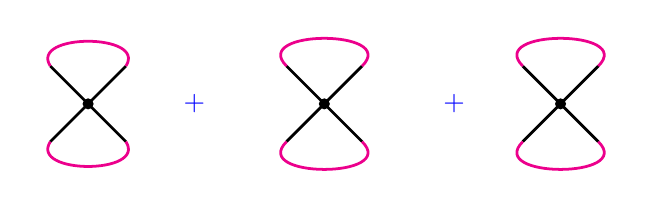
\begin{tikzpicture}[x=1cm,y=1cm]
  \foreach \x in {-3.0,0,3.0} {
    \fill (\x,0) circle (2pt);
    \draw[black,line width=1.0pt] (\x-0.48,-0.48)--(\x+0.48,0.48);
    \draw[black,line width=1.0pt] (\x-0.48,0.48)--(\x+0.48,-0.48);
  }
  \draw[magenta,line width=1.0pt] (-3.48,0.48) .. controls (-3.75,0.9)
    and (-2.25,0.9) .. (-2.52,0.48);
  \draw[magenta,line width=1.0pt] (-3.48,-0.48) .. controls (-3.75,-0.9)
    and (-2.25,-0.9) .. (-2.52,-0.48);
  \draw[blue] (-1.65,0) node {+};
  \draw[magenta,line width=1.0pt] (-0.48,0.48) .. controls (-0.95,0.95)
    and (0.95,0.95) .. (0.48,0.48);
  \draw[magenta,line width=1.0pt] (-0.48,-0.48) .. controls (-0.95,-0.95)
    and (0.95,-0.95) .. (0.48,-0.48);
  \draw[blue] (1.65,0) node {+};
  \draw[magenta,line width=1.0pt] (2.52,0.48) .. controls (2.05,0.95)
    and (3.95,0.95) .. (3.48,0.48);
  \draw[magenta,line width=1.0pt] (2.52,-0.48) .. controls (2.05,-0.95)
    and (3.95,-0.95) .. (3.48,-0.48);
\end{tikzpicture}
\end{center}

% AMBIGUITY P42-A1: retain the red Assume, the orange bracketed warning,
% the blue free-Wick annotation, the centered multiplication dots, and all
% three distinct quartic pairings. See work/253a-ch02/ambiguities.md.

% PAGE-TRANSITION: physical p. 42 ends with the order-g Wick pairings;
% physical p. 43 evaluates that term, begins the g^2 term, and leaves the
% graph-combinatorics sentence open at the lower edge.

% ---------------------------------------------------------------------------
\YinPageBoundary{32}{43}

\[
 =-\frac{g}{8}\int d\tau\,\bigl(G_0(\tau,\tau)\bigr)^2
\]
\begin{center}
\begin{tikzpicture}[>=Stealth]
  \draw[blue,->,line width=0.8pt] (0,-0.6)--(0,0.1);
  \draw[blue,line width=0.8pt,decorate,
    decoration={brace,amplitude=3pt,mirror}] (0.6,-0.05)--(2.6,-0.05);
  \node[blue] at (1.6,-0.55) {\textquotedblleft const\textquotedblright};
  \node[blue,align=left] at (1.55,-1.15)
    {diverges as $\tau\mathbin{->}\pm\infty$,\\[-1pt] will interpret later.};
\end{tikzpicture}
\end{center}

\YinLine{At order $g^2$.}
\[
 \frac{1}{2}\left(-\frac{g}{4!}\right)^2
 \int d\tau_1,d\tau_2\,
 \left\langle\bigl(\phi(\tau_1)\bigr)^4
 \bigl(\phi(\tau_2)\bigr)^4\right\rangle_0
\]

\YinLine{Two types of Wick contractions:}

\begin{center}
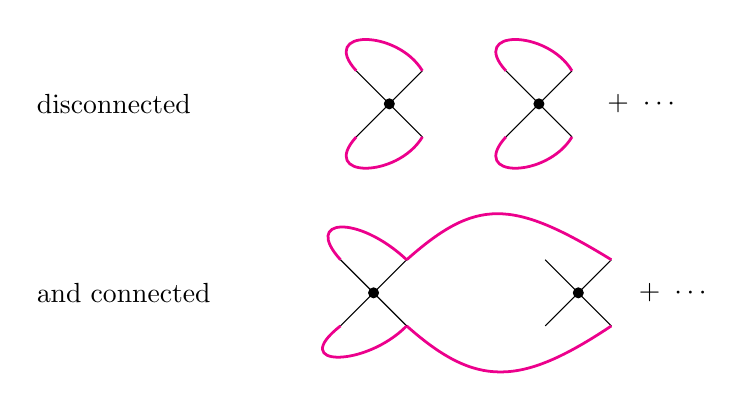
\begin{tikzpicture}[x=1cm,y=1cm]
  \node[anchor=west] at (-6.0,1.6) {disconnected};
  \foreach \x in {-1.4,0.5} {
    \fill (\x,1.6) circle (2pt);
    \draw[black] (\x-0.42,1.18)--(\x+0.42,2.02);
    \draw[black] (\x-0.42,2.02)--(\x+0.42,1.18);
    \draw[magenta,line width=1.0pt] (\x-0.42,2.02) .. controls
      (\x-0.9,2.55) and (\x+0.1,2.55) .. (\x+0.42,2.02);
    \draw[magenta,line width=1.0pt] (\x-0.42,1.18) .. controls
      (\x-0.9,0.65) and (\x+0.1,0.65) .. (\x+0.42,1.18);
  }
  \node at (1.8,1.6) {$+\ \cdots$};
  \node[anchor=west] at (-6.0,-0.8) {and connected};
  \foreach \x in {-1.6,1.0} {
    \fill (\x,-0.8) circle (2pt);
    \draw[black] (\x-0.42,-1.22)--(\x+0.42,-0.38);
    \draw[black] (\x-0.42,-0.38)--(\x+0.42,-1.22);
  }
  \draw[magenta,line width=1.0pt] (-2.02,-0.38) .. controls (-2.5,0.15)
    and (-1.8,0.2) .. (-1.18,-0.38);
  \draw[magenta,line width=1.0pt] (-2.02,-1.22) .. controls (-2.7,-1.75)
    and (-1.7,-1.75) .. (-1.18,-1.22);
  \draw[magenta,line width=1.0pt] (-1.18,-0.38) .. controls (-0.3,0.4)
    and (0.15,0.4) .. (1.42,-0.38);
  \draw[magenta,line width=1.0pt] (-1.18,-1.22) .. controls (-0.3,-2.0)
    and (0.25,-2.0) .. (1.42,-1.22);
  \node at (2.2,-0.8) {$+\ \cdots$};
\end{tikzpicture}
\end{center}

\YinLine{More generally, at order $g^n$,}
\YinLine{each set of Wick contractions can be}
\YinLine{represented by a graph that consists of}

% AMBIGUITY P43-A1: the blue quotation marks around ``const'', the brace
% endpoints, and the exact third connected pairing are visual readings only.
% See work/253a-ch02/ambiguities.md.
% AMBIGUITY P43-A2: the field glyph in the g^2 expectation is retained as
% phi/varphi according to the lane reading; no canonical replacement is made.
% See work/253a-ch02/ambiguities.md.

% PAGE-TRANSITION: physical p. 43 continues on physical p. 44 with K
% connected components and the multiplicities m_l.

% ---------------------------------------------------------------------------
\YinPageBoundary{33}{44}

\YinLine{K connected components, among them}
\YinLine{there are $m_\ell$ connected graphs that contain}
\YinLine{$\ell$ vertices each, $\ell=1,2,3,\ldots$}

\[
 \sum_{\ell\ge 1}m_\ell=K,\qquad
 \sum_{\ell\ge 1}m_\ell\cdot\ell=n.
\]
\begin{center}
\begin{tikzpicture}[>=Stealth]
  \draw[blue,->,line width=0.8pt] (0,0.3) .. controls (0.7,0.9)
    and (2.2,0.9) .. (3.0,0.3);
\end{tikzpicture}
\end{center}

\YinLine{For a given such partition of $n$,}
\YinLine{specified by $m_\ell$'s, the number of ways}
\YinLine{of grouping the $n$ vertices in this pattern}
\YinLine{is}
\[
 \frac{n!}{\prod_{\ell\ge 1}(\ell!)^{m_\ell}\cdot m_\ell!}
\]

\YinLine{Total contribution is}
\[
 \frac{1}{n!}
 \frac{n!}{\prod_{\ell\ge 1}(\ell!)^{m_\ell}\cdot m_\ell!}
 \prod_{\ell\ge 1}\left(G^{(\ell)}\right)^{m_\ell}
\]
\[
 =\prod_{\ell\ge 1}\frac{1}{m_\ell!}
 \left(\frac{1}{\ell!}G^{(\ell)}\right)^{m_\ell}
\]
\begin{center}
\begin{tikzpicture}[>=Stealth]
  \draw[blue,->,line width=0.8pt] (0,0)--(0.45,0.55);
\end{tikzpicture}
\end{center}

% AMBIGUITY P44-A1: retain the centered denominator dots and the scope of
% the product exactly as written. See work/253a-ch02/ambiguities.md.
% PAGE-TRANSITION: physical p. 44 points from G^{(ell)} to its definition on
% physical p. 45, where the partition sum is exponentiated.

% ---------------------------------------------------------------------------
\YinPageBoundary{34}{45}

% An isolated blue hooked stroke appears above the first annotation. It has no
% attached word or recoverable arrowhead.
\begin{center}
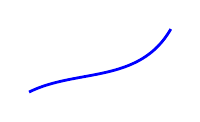
\begin{tikzpicture}
  \draw[blue,line width=1.0pt] (0,0) .. controls (0.6,0.3)
    and (1.4,0.1) .. (1.8,0.8);
\end{tikzpicture}
\end{center}

\begin{center}
\YinBlue{$G^{(\ell)}$ is the contribution from}\\[-2pt]
\YinBlue{connected Wick contraction of}\\[-2pt]
\YinBlue{$\ell$ vertices}
\end{center}

\[
 \frac{Z_g}{Z_0}
 =\sum_{\{m_\ell\}}\prod_{\ell\ge 1}
 \frac{1}{m_\ell!}\left(\frac{1}{\ell!}G^{(\ell)}\right)^{m_\ell}
\]
\[
 =\prod_{\ell\ge 1}\exp\left(\frac{1}{\ell!}G^{(\ell)}\right)
\]
\[
 =\exp\left(\sum_{\ell\ge 1}\frac{1}{\ell!}G^{(\ell)}\right)
\]

\begin{center}
\begin{tikzpicture}[>=Stealth]
  \draw[blue,line width=0.8pt,decorate,
    decoration={brace,amplitude=4pt,mirror}] (-2.0,0)--(2.0,0);
  \node[blue,align=center] at (0,-0.7)
    {contribution from all\\ connected graphs};
\end{tikzpicture}
\end{center}

\begin{center}
\YinBlue{$e.g.$}
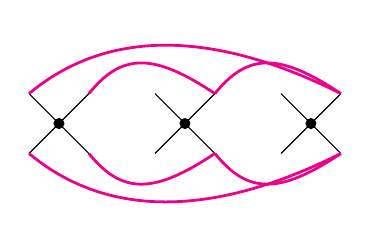
\begin{tikzpicture}[x=1cm,y=1cm]
  \foreach \x in {-1.6,0,1.6} {
    \fill (\x,0) circle (2pt);
    \draw[black] (\x-0.38,-0.38)--(\x+0.38,0.38);
    \draw[black] (\x-0.38,0.38)--(\x+0.38,-0.38);
  }
  \draw[magenta,line width=1.0pt] (-1.98,0.38) .. controls (-1.0,1.2)
    and (0.35,1.2) .. (1.98,0.38);
  \draw[magenta,line width=1.0pt] (-1.98,-0.38) .. controls (-1.0,-1.2)
    and (0.35,-1.2) .. (1.98,-0.38);
  \draw[magenta,line width=1.0pt] (-1.22,0.38) .. controls (-0.8,0.9)
    and (-0.4,0.9) .. (0.38,0.38);
  \draw[magenta,line width=1.0pt] (-1.22,-0.38) .. controls (-0.8,-0.9)
    and (-0.4,-0.9) .. (0.38,-0.38);
  \draw[magenta,line width=1.0pt] (0.38,0.38) .. controls (0.8,0.9)
    and (1.2,0.9) .. (1.98,0.38);
  \draw[magenta,line width=1.0pt] (0.38,-0.38) .. controls (0.8,-0.9)
    and (1.2,-0.9) .. (1.98,-0.38);
\end{tikzpicture}
\end{center}

\YinBlue{\[
\begin{aligned}
={}&\frac{1}{3!}\left(-\frac{g}{4!}\right)^3
 \int d\tau_1\,d\tau_2\,d\tau_3\,
 \left(G_0(\tau_1,\tau_2)\right)^2\\[-1pt]
&\cdot\left(G_0(\tau_2,\tau_3)\right)^2
 \left(G_0(\tau_3,\tau_1)\right)^2.
\end{aligned}
\]}

\YinBlue{\YinLine{Still diverges like $\int d\tau\cdot(\mathrm{Const})$.}}

% AMBIGUITY P45-A1: the isolated upper blue stroke and the case of
% ``Const'' are retained as open visual readings. See
% work/253a-ch02/ambiguities.md.

% PAGE-TRANSITION: physical p. 45 ends the connected-graph exponentiation
% example and begins a new heading, ``Interpretation of'', on physical p. 46.

% ---------------------------------------------------------------------------
\YinPageBoundary{35}{46}

\begin{center}
  Interpretation of
\end{center}

\[
\begin{aligned}
 Z&=\int [Dq]e^{-\int d\tau\,L^E}\\
  &=\langle q_f\,|\,e^{-HT}\,|\,q_i\rangle
\end{aligned}
\]

\begin{center}
\begin{tikzpicture}[>=Stealth]
  \draw[blue,->,line width=0.8pt] (-2.0,0)--(-1.3,0.35);
  \draw[blue,->,line width=0.8pt] (2.0,0)--(1.3,0.35);
  \node[blue,align=left] at (0,-0.15)
    {boundary\\ condition at initial and final\\
     imaginary time $\tau=0,T$,\\
     unspecified as we take $T\to\infty$};
\end{tikzpicture}
\end{center}

\[
 \log Z=-E_0\cdot T+O(1)
\]
\begin{center}
\begin{tikzpicture}[>=Stealth]
  \draw[blue,decorate,decoration={snake,amplitude=0.3mm,segment length=1.8mm}]
    (-0.3,0)--(0.5,0);
  \draw[blue,->] (0.1,-0.7)--(0.1,-0.05);
  \node[blue] at (0.1,-1.0) {ground state energy};
\end{tikzpicture}
\end{center}

\YinLine{Indeed, we have seen in perturbation}
\YinLine{theory.}
\[
 \log\frac{Z_g}{Z_0}=\sum_{\ell=1}^{\infty}\frac{1}{\ell!}G^{(\ell)}
\]
\begin{center}
\begin{tikzpicture}[>=Stealth]
  \draw[blue,decorate,decoration={snake,amplitude=0.3mm,segment length=1.8mm}]
    (-0.35,0)--(0.75,0);
  \draw[blue,->] (0.2,-0.65)--(0.2,-0.05);
  \node[blue,align=center] at (0.2,-1.05)
    {sum of all Wick contractions\\ of $\ell$ vertices via \underline{connected} graphs};
\end{tikzpicture}
\end{center}

\YinLine{$*$ One often absorbs the combinatorial}

% AMBIGUITY P46-A1: the endpoint arrows and the notation L^E are preserved
% without choosing a canonical boundary-condition convention. See
% work/253a-ch02/ambiguities.md.
% PAGE-TRANSITION: the starred sentence continues on physical p. 47 with
% ``factor 1/ell! into the "symmetry factor" of the graph itself.''

% ---------------------------------------------------------------------------
\YinPageBoundary{36}{47}

\YinLine{factor $\frac{1}{\ell!}$ into the \textquotedblleft symmetry factor\textquotedblright}
\YinLine{of the graph itself.}

\YinLine{$*$ each $G^{(\ell)}$ is of the form}
\[
 \int d\tau\,(\mathrm{const})\propto T.
\]

\YinLine{Thus}
\[
 E_0=-\lim_{T\to\infty}\frac{1}{T}\log Z
\]
\YinLine{is well-defined.}

\YinLine{As already seen, at order $g$, $\ell=1$.}

\begin{center}
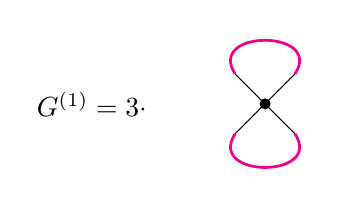
\begin{tikzpicture}[baseline]
  \node at (-1.2,0) {$G^{(1)}=3\cdot$};
  \fill (1.0,0) circle (2pt);
  \draw[black] (0.62,-0.38)--(1.38,0.38);
  \draw[black] (0.62,0.38)--(1.38,-0.38);
  \draw[magenta,line width=1.0pt] (0.62,0.38) .. controls (0.25,0.95)
    and (1.75,0.95) .. (1.38,0.38);
  \draw[magenta,line width=1.0pt] (0.62,-0.38) .. controls (0.25,-0.95)
    and (1.75,-0.95) .. (1.38,-0.38);
\end{tikzpicture}
\end{center}

\[
 =-\frac{g}{8}\cdot\int d\tau\,\bigl(G_0(\tau,\tau)\bigr)^2
\]

\begin{center}
\YinBlue{Recall}\qquad
\YinBlue{$G(\tau_1,\tau_2)=\frac{1}{2\omega}e^{-\omega|\tau_{12}|}$}
\\[4pt]
\YinBlue{$G_0(\tau,\tau)=\frac{1}{2\omega}$}
\end{center}

\[
 \Rightarrow\Delta E_0=\frac{g}{8}\cdot
 \left(\frac{1}{2\omega}\right)^2+O(g^2)
\]
\begin{center}
\begin{tikzpicture}[>=Stealth]
  \draw[blue,->] (0,0.45)--(0,0.05);
  \node[blue] at (1.3,0.4) {correction to ground state energy};
  \node[gray] at (3.2,1.0) {(have set $\omega=1$)};
\end{tikzpicture}
\end{center}

% AMBIGUITY P47-A1: the first blue propagator reminder is G rather than G_0
% in the source capture; the case of const and the exact loop strokes remain
% open. See work/253a-ch02/ambiguities.md.
% PAGE-TRANSITION: physical p. 47 ends with the path-integral energy shift;
% physical p. 48 begins ``Comparison to Hamiltonian perturbation theory:''.

% ---------------------------------------------------------------------------
\YinPageBoundary{37}{48}

\begin{center}
  Comparison to Hamiltonian perturbation theory:
\end{center}

% A small isolated black dot sits immediately before the Hamiltonian line.
\YinLine{$\cdot\quad H=\frac{\widehat p^{\,2}}{2}+\frac{\widehat q^{\,2}}{2}
 +\frac{1}{4!}g\widehat q^{\,4}$}

\begin{center}
\begin{tikzpicture}[>=Stealth]
  \draw[blue,line width=0.8pt,decorate,
    decoration={brace,amplitude=4pt,mirror}] (-2.8,0)--(-0.2,0);
  \node[blue] at (-1.5,-0.45) {$H_0$};
  \draw[blue,line width=0.8pt,decorate,
    decoration={brace,amplitude=4pt,mirror}] (0.35,0)--(2.7,0);
  \node[blue] at (1.5,-0.45) {$H_1$};
\end{tikzpicture}
\end{center}

\YinLine{Let $|\psi_0\rangle$ be ground state of $H_0$,}
\YinLine{to leading order in $g$,}
\[
\begin{aligned}
 \Delta E_0&\approx\langle\psi_0|H_1|\psi_0\rangle\\
 &=\frac{1}{4!}g\left\langle\widehat q^{\,4}\right\rangle_0
 =\frac{g}{32}.
\end{aligned}
\]
\begin{center}
\begin{tikzpicture}
  \draw[blue,line width=0.8pt,decorate,
    decoration={brace,amplitude=3pt,mirror}] (-1.6,0)--(0.1,0);
  \node[blue] at (-0.75,-0.45) {$=\frac{3}{4}$};
  \node[blue] at (1.4,0.1) {$\checkmark$};
\end{tikzpicture}
\end{center}

% AMBIGUITY P48-A1: retain the isolated black dot and the three short blue
% brace-to-label strokes as source marks, not algebraic symbols. See
% work/253a-ch02/ambiguities.md.
% PAGE-TRANSITION: physical p. 48 closes the first-order comparison at g/32;
% physical p. 49 turns to the positive-time two-point function.

% ---------------------------------------------------------------------------
\YinPageBoundary{38}{49}

\YinLine{Next we turn to}\hfill\YinLine{$(\tau>0)$}

\[
 \left\langle0\middle|\widehat q(\tau)\widehat q(0)\middle|0\right\rangle
\]
\[
 =\frac{1}{Z}\int[Dq]e^{-\int d\tau\,L^E}\cdot q(\tau)q(0).
\]

\begin{center}
\begin{tikzpicture}[>=Stealth]
  \draw[magenta,->,line width=0.9pt] (0,-1.0) .. controls (0.2,-0.4)
    and (0.9,-0.2) .. (1.1,0.25);
  \node[magenta] at (0,-1.35) {expand in $g$.};
\end{tikzpicture}
\end{center}

\[
 =\frac{1}{Z}\left\langle q(\tau)q(0)
 \sum_{n=0}^{\infty}\frac{1}{n!}
 \left(-\frac{g}{4!}\int d\tau'\,q^4(\tau')\right)^n
 \right\rangle_{\YinBlue{0}}.
\]

\begin{center}
\begin{tikzpicture}[>=Stealth]
  \draw[blue,->,line width=0.8pt] (-0.8,-0.8)--(-0.2,0.0);
  \node[blue,align=left] at (0,-1.45)
    {Computed by summing up all possible\\
     Wick contractions, consisting of terms\\ like};
\end{tikzpicture}
\end{center}

\[
 q(\tau)q(0)\left(-\frac{g}{4!}\int d\tau'\,q^4(\tau')\right)
 \left(\text{graphical Wick-contraction pattern}\right)\cdots
\]

% The purple overbrackets group the external fields, the interaction, and
% successive contraction choices. The grouped symbols are retained even
% though the individual pairings are not separately labeled in the source.
\begin{center}
\begin{tikzpicture}[x=1cm,y=1cm,>=Stealth]
  \fill[red] (-3.5,0) circle (2.5pt);
  \fill[red] (0.0,0) circle (2.5pt);
  \draw[black,line width=1.0pt] (-3.5,0)--(0,0);
  \fill ( -1.75,0) circle (2pt);
  \draw[magenta,line width=1.0pt] (-1.75,0) .. controls (-2.3,0.9)
    and (-1.2,0.9) .. (-1.75,0);
  \node[red] at (-3.5,-0.45) {$x(\tau)$};
  \node[red] at (0,-0.45) {$x(0)$};
  \draw[blue,line width=0.8pt,decorate,
    decoration={brace,amplitude=4pt,mirror}] (1.3,0.5)--(4.0,0.5);
  \node[blue,align=left] at (2.7,-0.7)
    {other disconnected\\ component of\\ the graph};
\end{tikzpicture}
\end{center}

\YinLine{The sum factorizes as}
\begin{center}
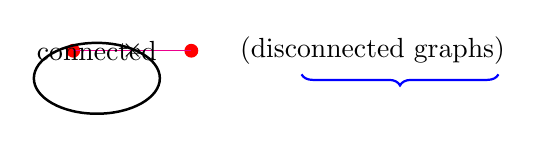
\begin{tikzpicture}[x=1cm,y=1cm]
  \fill[red] (-3.3,0) circle (2.5pt);
  \fill[red] (-1.8,0) circle (2.5pt);
  \draw[magenta] (-3.3,0)--(-1.8,0);
  \draw[black,line width=0.9pt] (-3.0,-0.35) ellipse (0.8 and 0.45);
  \node at (-3.0,0) {connected};
  \node at (-2.55,0) {$\times$};
  \node at (0.5,0) {(disconnected graphs)};
  \draw[blue,line width=0.8pt,decorate,
    decoration={brace,amplitude=4pt,mirror}] (-0.4,-0.3)--(2.1,-0.3);
\end{tikzpicture}
\end{center}

% AMBIGUITY P49-A1: the red endpoint labels in the connected example are
% captured as x(tau), x(0), although the surrounding equations use q. See
% work/253a-ch02/ambiguities.md.
% PAGE-TRANSITION: physical p. 49 leaves the connected/disconnected
% factorization open; physical p. 50 begins with Z cancelling 1/Z.

% ---------------------------------------------------------------------------
\YinPageBoundary{39}{50}

\begin{center}
\YinBlue{\textquotedblleft Z\textquotedblright}\\[-2pt]
\YinBlue{Cancels against $\frac{1}{Z}$.}
\end{center}
\YinLine{leaving the result}
\[
 \left\langle0\middle|\widehat q(\tau)\widehat q(0)\middle|0\right\rangle
\]

% The source displays the connected diagram series rather than symbolic
% names. The endpoint dots are red and the graph strokes are black.
\begin{center}
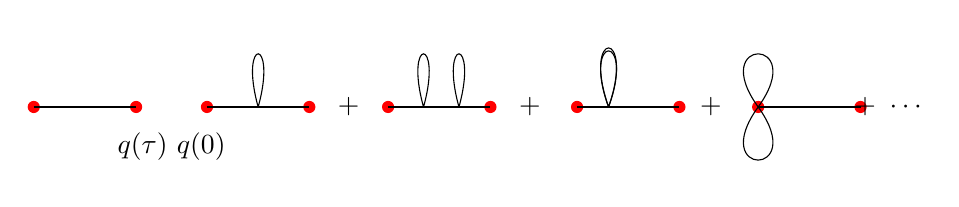
\begin{tikzpicture}[x=1cm,y=1cm]
  \foreach \x in {-5.2,-3.0,-0.7,1.7,4.0} {
    \fill[red] (\x-0.65,0) circle (2.2pt);
    \fill[red] (\x+0.65,0) circle (2.2pt);
    \draw[black] (\x-0.65,0)--(\x+0.65,0);
  }
  \draw[black] (-3.0,0) .. controls (-3.25,0.9) and (-2.75,0.9) .. (-3.0,0);
  \draw[black] (-0.9,0) .. controls (-1.15,0.9) and (-0.65,0.9) .. (-0.9,0);
  \draw[black] (-0.45,0) .. controls (-0.7,0.9) and (-0.2,0.9) .. (-0.45,0);
  \draw[black] (1.45,0) .. controls (1.1,0.95) and (1.8,0.95) .. (1.45,0);
  \draw[black] (1.45,0) .. controls (1.1,1.0) and (1.8,1.0) .. (1.45,0);
  \draw[black] (3.35,0) .. controls (2.7,-0.9) and (4.0,-0.9) .. (3.35,0);
  \draw[black] (3.35,0) .. controls (2.7,0.9) and (4.0,0.9) .. (3.35,0);
  \node at (-4.1,-0.5) {$q(\tau)\ q(0)$};
  \node at (-1.85,0) {$+$};
  \node at (0.45,0) {$+$};
  \node at (2.75,0) {$+$};
  \node at (5.0,0) {$+\ \cdots$};
\end{tikzpicture}
\end{center}

\YinGray{\YinLine{Note: Same path integral expression computes}}
\YinGray{\[
 \left\langle0\middle|\widehat q(0)\widehat q(\tau)\middle|0\right\rangle
 \qquad\text{for $\tau<0$.}
\]}
\YinGray{\YinLine{We can write the Euclidean Green function}}
\YinGray{\[
 \left\langle q(\tau)q(0)\right\rangle=
 \begin{cases}
  \left\langle0\middle|\widehat q(\tau)\widehat q(0)\middle|0\right\rangle,
    &\tau\ge0,\\[4pt]
  \left\langle0\middle|\widehat q(0)\widehat q(\tau)\middle|0\right\rangle,
    &\tau<0.
 \end{cases}
\]}

\begin{center}
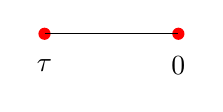
\begin{tikzpicture}
  \fill[red] (0,0) circle (2.2pt); \fill[red] (1.7,0) circle (2.2pt);
  \draw (0,0)--(1.7,0);
  \node at (0,-0.4) {$\tau$}; \node at (1.7,-0.4) {$0$};
\end{tikzpicture}
\end{center}
\[
 G_0(\tau)=\frac{1}{2}e^{-|\tau|}
\]
\YinBlue{\[
 =\int\frac{dk}{2\pi}\,\widetilde G_0(k)e^{ik\tau},
 \qquad \widetilde G_0(k)=\frac{1}{k^2+1}
\]}

% AMBIGUITY P50-A1: preserve the source distinction tau>0 on p. 49 and
% tau>=0 in the first branch here, and preserve the diagrammatic series.
% See work/253a-ch02/ambiguities.md.
% PAGE-TRANSITION: physical p. 50 ends with G_0(tau) and its Fourier form;
% physical p. 51 begins the one-loop tadpole evaluation.

% ---------------------------------------------------------------------------
\YinPageBoundary{40}{51}

\begin{center}
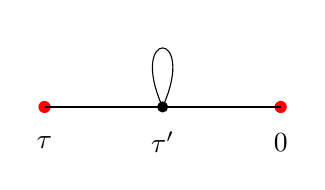
\begin{tikzpicture}
  \fill[red] (0,0) circle (2.2pt); \fill[red] (3.0,0) circle (2.2pt);
  \draw (0,0)--(3.0,0); \fill (1.5,0) circle (2pt);
  \draw (1.5,0) .. controls (1.05,1.0) and (1.95,1.0) .. (1.5,0);
  \node at (0,-0.45) {$\tau$}; \node at (1.5,-0.45) {$\tau'$};
  \node at (3.0,-0.45) {$0$};
\end{tikzpicture}
\end{center}
\[
 =-\frac{g}{2}\int d\tau'\,G_0(\tau-\tau')G_0(\tau')G_0(0)
\]

\YinLine{convenient to evaluation using Fourier transf.}
\[
\begin{aligned}
={}&-\frac{g}{2}\int d\tau'\int\frac{dk}{2\pi}\int\frac{dk'}{2\pi}
 \widetilde G_0(k)\widetilde G_0(k')
 e^{ik(\tau-\tau')+ik'\tau'}\\[-1pt]
&\cdot\int\frac{dk''}{2\pi}\cdot\widetilde G_0(k'')
\end{aligned}
\]
\[
 =-\frac{g}{2}\cdot\frac{1}{2}\int\frac{dk}{2\pi}\cdot
 \frac{e^{ik\tau}}{(k^2+1)^2}
\]

\begin{center}
\begin{tikzpicture}[>=Stealth]
  \fill (0,0) circle (2pt); \fill (2.6,0) circle (2pt);
  \draw (0,0)--(2.6,0); \fill (1.3,0) circle (2pt);
  \draw (1.3,0) .. controls (0.85,0.9) and (1.75,0.9) .. (1.3,0);
  \draw[blue,->] (0.85,-0.28)--(0.35,-0.28);
  \draw[blue,->] (2.15,-0.28)--(1.65,-0.28);
  \draw[blue,->] (1.0,0.75)--(0.82,0.35);
  \node[blue] at (0.55,-0.65) {$k$};
  \node[blue] at (2.05,-0.65) {$k'=k$};
  \node[blue] at (1.0,1.05) {$k''$};
\end{tikzpicture}
\end{center}

\YinLine{At order $g^2$, we have}
\begin{center}
\begin{tikzpicture}[x=1cm,y=1cm]
  \foreach \x in {-3.0,0,3.0} {
    \fill[red] (\x-0.7,0) circle (2pt); \fill[red] (\x+0.7,0) circle (2pt);
    \draw (\x-0.7,0)--(\x+0.7,0);
  }
  \draw (-3.0,0) .. controls (-3.35,0.9) and (-2.65,0.9) .. (-3.0,0);
  \draw (-2.55,0) .. controls (-2.9,0.9) and (-2.2,0.9) .. (-2.55,0);
  \draw (0,0) .. controls (-0.45,0.95) and (0.45,0.95) .. (0,0);
  \draw (0,0) .. controls (-0.65,-0.95) and (0.65,-0.95) .. (0,0);
  \draw (3.0,0) .. controls (2.2,1.0) and (3.8,1.0) .. (3.0,0);
  \draw (3.0,0) .. controls (2.2,-1.0) and (3.8,-1.0) .. (3.0,0);
\end{tikzpicture}
\end{center}

\begin{center}
\YinGreen{$[\text{Calculate these in Pset 2}]$}
\end{center}

\YinLine{The full (perturbative) 2-point function}
\YinLine{$\langle q(\tau)q(0)\rangle$ has the structure}

% AMBIGUITY P51-A1: the source uses unaccented q in the lower boundary line,
% while the preceding operator correlator has hats. Preserve both readings.
% The three g^2 graphs and the momentum-routing arrows remain source objects.
% See work/253a-ch02/ambiguities.md.
% PAGE-TRANSITION: physical p. 51 opens the full two-point-function structure;
% physical p. 52 expands it into free and 1PI insertions.

% ---------------------------------------------------------------------------
\YinPageBoundary{41}{52}

% Full two-point diagram and its 1PI expansion. The large hatched oval is the
% source symbol for the full perturbative two-point function.
\begin{center}
\begin{tikzpicture}[x=1cm,y=1cm,>=Stealth]
  \fill[red] (-6.2,0) circle (2pt); \fill[red] (-5.1,0) circle (2pt);
  \draw (-6.2,0)--(-5.1,0);
  \draw[black,line width=1.0pt] (-5.95,-0.5) ellipse (0.72 and 0.5);
  \foreach \y in {-0.3,0,0.3} {\draw (-6.25,\y-0.2)--(-5.65,\y+0.2);}
  \node at (-4.6,0) {$=$};
  \fill[red] (-4.0,0) circle (2pt); \fill[red] (-2.6,0) circle (2pt);
  \draw (-4.0,0)--(-2.6,0); \node[blue] at (-3.3,0.45) {$G_0$};
  \node at (-2.15,0) {$+$};
  \fill[red] (-1.6,0) circle (2pt); \fill[red] (0.7,0) circle (2pt);
  \draw (-1.6,0)--(0.7,0);
  \draw[black,line width=1.0pt] (-0.45,0) ellipse (0.75 and 0.42);
  \node at (-0.45,0) {1PI};
  \node[blue] at (-1.2,0.45) {$G_0$}; \node[blue] at (0.25,0.45) {$G_0$};
  \node at (1.15,0) {$+$};
  \fill[red] (1.7,0) circle (2pt); \fill[red] (5.0,0) circle (2pt);
  \draw (1.7,0)--(5.0,0);
  \draw[black,line width=1.0pt] (2.7,0) ellipse (0.62 and 0.42);
  \draw[black,line width=1.0pt] (4.0,0) ellipse (0.62 and 0.42);
  \node at (2.7,0) {1PI}; \node at (4.0,0) {1PI};
  \node at (5.55,0) {$+\ \cdots$};
\end{tikzpicture}
\end{center}

\begin{center}
\begin{tikzpicture}[>=Stealth]
  \draw[magenta,->,line width=0.9pt] (0.3,1.2)--(0.3,0.55);
  \node[magenta] at (1.6,1.2)
    {\textquotedblleft 1-particle-irreducible\textquotedblright};
\end{tikzpicture}
\end{center}

\begin{center}
\begin{tikzpicture}[>=Stealth]
  \draw[gray,line width=0.9pt] (-3.3,0)--(3.3,0);
  \node[gray,align=center] at (0,1.0)
    {would remain connected after cutting\\ one propagator, i.e.};
  \draw[gray,line width=0.8pt] (-1.6,-0.35)--(-0.1,-0.35);
  \draw[gray] (-0.85,-0.35) .. controls (-1.2,0.35) and (-0.5,0.35) .. (-0.85,-0.35);
  \draw[gray,line width=0.8pt] (0.7,-0.35)--(2.2,-0.35);
  \draw[gray] (1.45,-0.35) ellipse (0.5 and 0.35);
  \draw[gray] (1.45,-0.62)--(1.45,-0.1);
\end{tikzpicture}
\end{center}

\[
 =\int\frac{dk}{2\pi}e^{ik\tau}\widetilde G_0(k)
 \sum_{n=0}^{\infty}\left(\widetilde G_0(k)\cdot\Sigma(k)\right)^n
\]
\[
 =\int\frac{dk}{2\pi}e^{ik\tau}
 \frac{1}{k^2+1-\Sigma(k)}
\]

\begin{center}
\begin{tikzpicture}[>=Stealth]
  \node at (-1.5,0) {$\Sigma(k)=$};
  \draw[gray] (-0.2,0)--(0.7,0);
  \draw[black,line width=1.0pt] (0.7,0) ellipse (0.7 and 0.45);
  \node at (0.7,0) {1PI};
  \draw[gray] (1.4,0)--(2.3,0);
  \draw[magenta,->] (-0.1,-0.7)--(0.25,-0.1);
  \draw[magenta,->] (2.2,-0.7)--(1.75,-0.1);
  \node[blue] at (0.0,0.45) {$k$}; \node[blue] at (2.0,0.45) {$k$};
  \node[magenta,align=center] at (1.0,-1.15)
    {not including external propagators\\
     \textquotedblleft amputated graph\textquotedblright};
\end{tikzpicture}
\end{center}

\begin{center}
\begin{tikzpicture}[x=1cm,y=1cm]
  \draw[gray] (-3.3,0)--(-2.0,0);
  \draw[black] (-2.0,0) .. controls (-2.45,0.95) and (-1.55,0.95) .. (-2.0,0);
  \node at (-1.6,0) {$+$};
  \draw[gray] (-1.1,0)--(0.2,0);
  \draw[black] (-0.45,0) .. controls (-0.85,0.9) and (-0.05,0.9) .. (-0.45,0);
  \draw[black] (-0.45,0) .. controls (-1.0,-0.9) and (0.1,-0.9) .. (-0.45,0);
  \node at (0.65,0) {$+$};
  \draw[gray] (1.1,0)--(3.8,0);
  \draw[black] (1.9,0) .. controls (1.2,0.9) and (2.6,0.9) .. (1.9,0);
  \draw[black] (2.9,0) .. controls (2.2,-0.9) and (3.6,-0.9) .. (2.9,0);
  \node at (4.3,0) {$+\ \cdots$};
\end{tikzpicture}
\end{center}
\begin{center}
\YinGreen{\begin{tikzpicture}[>=Stealth]
  \draw[green!50!black,line width=0.8pt,decorate,
    decoration={brace,amplitude=4pt,mirror}] (-1.0,0)--(3.5,0);
  \node[green!50!black] at (1.2,-0.55) {homework};
\end{tikzpicture}}
\end{center}

\[
 =-\frac{g}{4}+\frac{g^2}{8}\left(\frac{1}{4}+\frac{1}{k^2+9}\right)
 +O(g^3).
\]

% AMBIGUITY P52-A1: the exact dot count in the diagrammatic ellipses, the
% interior hatch marks, and the two gray connectedness sketches are retained
% at topology level only. See work/253a-ch02/ambiguities.md.
% PAGE-TRANSITION: physical p. 52 ends the self-energy calculation; physical
% p. 53 begins ``In conclusion:'' and the complex-k-plane pole discussion.

% ---------------------------------------------------------------------------
\YinPageBoundary{42}{53}

\YinLine{In conclusion :}
\[
 \langle q(\tau)q(0)\rangle\equiv G(\tau)
 =\int\frac{dk}{2\pi}\,\widetilde G(k)e^{ik\tau}
\]
\[
 \widetilde G(k)=\frac{1}{k^2+1+\frac{g}{4}
 -\frac{g^2}{8}\left(\frac{1}{4}+\frac{1}{k^2+9}\right)+O(g^3)}.
\]

\YinLine{On the other hand, we know}
\[
 \left\langle0\middle|\widehat q(\tau)\widehat q(0)\middle|0\right\rangle
 \qquad(\text{for }\tau>0)
\]
\[
 =\sum_n\left|\left\langle n\middle|\widehat q(0)\middle|0\right\rangle\right|^2
 e^{-(\bar E_n-\bar E_0)\tau}.
\]

\YinLine{Consider the analytic continuation of}
\YinLine{$\widetilde G(k)$ to the complex $k$-plane:}

\begin{center}
\begin{tikzpicture}[x=1cm,y=1cm,>=Stealth]
  \draw[black,line width=0.8pt] (-3.2,-2.3) .. controls (-3.35,0)
    and (-3.1,2.3) .. (-2.8,2.5) -- (2.9,2.5)
    .. controls (3.25,0.5) and (3.0,-1.8) .. (3.0,-2.3)
    -- (-3.2,-2.3);
  \node[anchor=west] at (-3.0,2.1) {$k$};
  \draw[black] (-3.0,2.0)--(-2.4,2.0);
  \draw[blue,line width=0.9pt] (-3.2,0)--(3.0,0);
  \draw[blue,->,line width=0.9pt] (-0.2,0)--(0.9,0);
  \node[blue,anchor=west] at (3.0,0) {$\operatorname{Re}k$};
  \draw[green!50!black,line width=1.0pt] (-3.0,0) .. controls (-2.2,2.8)
    and (2.3,2.8) .. (3.0,0);
  \draw[green!50!black,->] (-2.4,1.75)--(-2.55,1.4);
  \node[red] at (-1.2,1.6) {poles};
  \node[red] at (-0.9,1.9) {$\times$};
  \node[red] at (-0.9,1.0) {$\times$};
  \node[purple] at (-0.1,1.9) {$i\omega_2$};
  \node[purple] at (-0.1,1.0) {$i\omega_1$};
  \node[red] at (-0.9,-0.9) {$\times$};
  \node[red] at (-0.9,-1.7) {$\times$};
  \node[red] at (-0.9,2.25) {$\vdots$};
  \node[red] at (-0.9,-2.05) {$\vdots$};
\end{tikzpicture}
\end{center}

% AMBIGUITY P53-A1: retain the underlined black k stroke, the Re k label,
% the unlabeled lower poles, and the absence of an Im k axis label. See
% work/253a-ch02/ambiguities.md.
% PAGE-TRANSITION: physical p. 53 leaves the contour sketch open; physical
% p. 54 closes the contour in the UHP and starts Example 3.

% ---------------------------------------------------------------------------
\YinPageBoundary{43}{54}

\YinLine{Closing the contour at infinity on UHP.}
\[
 \int\frac{dk}{2\pi}\,\widetilde G(k)e^{ik\tau}
 =i\sum_n e^{-\omega_n\tau}
 \underset{k\to i\omega_n}{\operatorname{Res}}\,\widetilde G(k)
\]

\begin{center}
\begin{tikzpicture}
  \node[draw=blue,line width=0.9pt,inner sep=7pt]
    {$\omega_n=\bar E_n-\bar E_0$};
\end{tikzpicture}
\end{center}

\YinLine{$e.g.$ from}
\[
 \widetilde G(k)=\frac{1}{k^2+1+\frac{g}{4}
 -\frac{g^2}{8}\left(\frac{1}{4}+\frac{1}{k^2+9}\right)
 +\ldotp\ldotp\ldotp\ldotp,}
\]
\YinLine{we expect the first pole to be near $k\simeq i$,}
\[
 \omega_1=1+\frac{g}{8}-\frac{g^2}{32}+O(g^3).
\]
\begin{center}
\begin{tikzpicture}
  \node[blue] at (0,0) {$\checkmark$};
  \node[green!50!black,draw=green!50!black,inner sep=5pt,align=center]
    at (2.2,0) {[agrees with Hamiltonian perturbation\\ theory at second order]};
\end{tikzpicture}
\end{center}

\begin{center}
\begin{tikzpicture}
  \draw[line width=0.8pt] (-5,0)--(5,0);
  \draw[line width=0.8pt] (4.55,0)--(4.55,0.2);
  \draw[line width=0.8pt] (4.8,0)--(4.8,0.2);
\end{tikzpicture}
\end{center}

\begin{center}
  \underline{Example 3:}
\end{center}
\[
 L=\frac{1}{2}\dot q^{\,2}-\frac{1}{2}q^2-\frac{g}{8}q^2\dot q^{\,2}
\]
\[
 p=\frac{\partial L}{\partial\dot q}
 =\dot q\left(1-\frac{g}{4}q^2\right)
\]
\[
 H=\dot q\,p-L
\]
\[
 =\frac{1}{2}\left(1-\frac{g}{4}q^2\right)^{-1}p^2+\frac{1}{2}q^2.
\]

% AMBIGUITY P54-A1: the repeated dots and comma after the example denominator,
% the two right-hand divider marks, and the exact Res placement remain open.
% See work/253a-ch02/ambiguities.md.
% PAGE-TRANSITION: physical p. 54 leaves Example 3 open after H; physical
% p. 55 changes variables and asks ``ordering in quantization ?''.

% ---------------------------------------------------------------------------
\YinPageBoundary{44}{55}

\begin{center}
\begin{tikzpicture}[>=Stealth]
  \draw[magenta,->,line width=0.9pt] (0,0)--(0.3,0.55);
  \node[magenta] at (1.5,0.45) {ordering in quantization ?};
\end{tikzpicture}
\end{center}

\YinGray{\YinLine{$*$ Can also consider a change of variable}}
\[
 \dot y=\sqrt{1-\frac{g}{4}\phi^2}\,\dot\phi
\]
\[
 y=\phi-\frac{g}{24}\phi^3+\cdots
\]
\YinGray{\YinLine{and rewrite $L\longrightarrow L(y,\dot y)$}}
\[
 =\frac{\dot y^{\,2}}{2}-V(y),
\]
\[
 V(y)=\frac{1}{2}y^2+\frac{g}{24}y^4+\cdots
\]
\YinGray{\YinLine{Same as anharmonic oscillator up}}
\YinGray{\YinLine{to $O(g^2)$ corrections to the potential.}}

\YinGray{\YinLine{But, we will insist on working with the}}
\YinGray{\YinLine{$\phi$-variable in the path integral, and}}
\YinGray{\YinLine{see what happens ...}}

% AMBIGUITY P55-A1: the magenta question and its upward arrow have no
% recoverable referent. The phi/varphi glyph is retained as phi. See
% work/253a-ch02/ambiguities.md.
% PAGE-TRANSITION: physical p. 55 turns from the change of variable back to
% the phi-variable in the path integral; physical p. 56 begins its Euclidean
% Lagrangian and integration-by-parts decomposition.

% ---------------------------------------------------------------------------
\YinPageBoundary{45}{56}

\[
 L^E=\frac{1}{2}(\partial_\tau\phi)^2+\frac{1}{2}\phi^2
 -\frac{1}{8}g\phi^2(\partial_\tau\phi)^2
\]
\begin{center}
\begin{tikzpicture}
  \draw[purple,line width=0.9pt,decorate,
    decoration={brace,amplitude=4pt,mirror}] (-1.0,0)--(2.8,0);
  \node[purple] at (0.9,-0.45) {\textquotedblleft\ \textquotedblright};
\end{tikzpicture}
\end{center}

\YinPurple{\[
 -\frac{g}{24}\partial_\tau(\phi^3\partial_\tau\phi)
 +\frac{g}{24}\phi^3\partial_\tau^2\phi
\]}
\begin{center}
\begin{tikzpicture}
  \draw[magenta,line width=0.8pt,decorate,
    decoration={brace,amplitude=3pt,mirror}] (-2.7,0)--(-0.1,0);
  \node[magenta] at (-1.4,-0.45) {total derivative};
  \node[magenta] at (-0.9,-0.9) {does not contribute to $S^E$};
  \draw[red,line width=0.8pt,decorate,
    decoration={brace,amplitude=3pt,mirror}] (0.3,0)--(2.7,0);
  \node[red] at (1.5,-0.45) {can keep just this};
\end{tikzpicture}
\end{center}

\YinLine{up to first order in $g$,}
\[
 \langle\phi(\tau)\,\phi(0)\rangle
\]
\begin{center}
\begin{tikzpicture}[x=1cm,y=1cm]
  \fill (0,0) circle (2pt); \fill (1.3,0) circle (2pt);
  \draw (0,0)--(1.3,0); \node at (0.65,-0.4) {$G_0(\tau)$};
  \node at (2.1,0) {$+$};
  \fill (2.8,0) circle (2pt); \fill (4.1,0) circle (2pt);
  \draw (2.8,0)--(4.1,0); \fill (3.45,0) circle (2pt);
  \draw (3.45,0) .. controls (3.0,0.95) and (3.9,0.95) .. (3.45,0);
  \draw[blue,->] (3.0,-0.8)--(3.4,-0.1);
  \node at (4.8,0) {$+\ \cdots$};
\end{tikzpicture}
\end{center}

\YinBlue{\[
 \phi(\tau)\,\phi(0)\cdot\frac{g}{8}
 \int d\tau'\,(\phi(\tau'))^2(\partial_{\tau'}\phi(\tau'))^2
\]}
\begin{center}
\begin{tikzpicture}
  \draw[magenta,line width=0.8pt,decorate,
    decoration={brace,amplitude=3pt,mirror}] (-3.4,0)--(2.8,0);
  \draw[magenta,line width=0.8pt,decorate,
    decoration={brace,amplitude=3pt,mirror}] (-1.0,0.18)--(1.5,0.18);
  \draw[magenta,line width=0.8pt,decorate,
    decoration={brace,amplitude=3pt,mirror}] (2.0,0.18)--(3.4,0.18);
\end{tikzpicture}
\end{center}
\YinMagenta{\YinLine{+ various other contractions}}
\YinLine{Can represent as several diagrams}
\begin{center}
\begin{tikzpicture}[>=Stealth]
  \draw[->,line width=0.8pt] (0,0)--(1.0,0.85);
\end{tikzpicture}
\end{center}

% Six lower one-vertex line-and-loop drawings. The blue marks are derivative
% insertions; the first drawing retains the tau, tau', 0 labels and arrow.
\begin{center}
\begin{tikzpicture}[x=1cm,y=1cm]
  \foreach \x/\y in {0/0,2.0/0,4.0/0,4.0/-1.5,6.0/0,6.0/-1.5} {
    \fill (\x,\y) circle (2pt); \fill (\x+1.2,\y) circle (2pt);
    \draw (\x,\y)--(\x+1.2,\y); \fill (\x+0.6,\y) circle (2pt);
    \draw (\x+0.6,\y) .. controls (\x+0.2,\y+0.85)
      and (\x+1.0,\y+0.85) .. (\x+0.6,\y);
  }
  \draw[blue] (0.35,0.16)--(0.35,-0.16); \draw[blue] (0.85,0.16)--(0.85,-0.16);
  \draw[blue] (2.35,0.16)--(2.35,-0.16); \draw[blue] (2.85,0.16)--(2.85,-0.16);
  \draw[blue] (4.35,0.16)--(4.35,-0.16); \draw[blue] (4.85,0.16)--(4.85,-0.16);
  \draw[blue] (6.35,0.16)--(6.35,-0.16); \draw[blue] (6.85,0.16)--(6.85,-0.16);
  \node at (0,-0.45) {$\tau$}; \node at (0.6,-0.45) {$\tau'$};
  \node at (1.2,-0.45) {$0$};
  \node[blue] at (0.6,-0.9) {$\uparrow$};
  \node at (1.6,0) {$+$}; \node at (3.6,0) {$+$};
  \node at (5.6,0) {$+$};
\end{tikzpicture}
\end{center}

% AMBIGUITY P56-A1: the purple brace-like mark under the interaction and the
% exact derivative-leg assignment in the six diagrams are visual readings.
% See work/253a-ch02/ambiguities.md.
% PAGE-TRANSITION: physical p. 56 ends with the first-order contraction row;
% physical p. 57 begins with the explicit 2-times contraction.

% ---------------------------------------------------------------------------
\YinPageBoundary{46}{57}

% A disconnected tall blue curved continuation stroke sits at the upper left.
\begin{center}
\begin{tikzpicture}
  \draw[blue,line width=1.0pt] (0,0.8) .. controls (-0.35,0.4)
    and (-0.35,-0.1) .. (0,-0.45);
\end{tikzpicture}
\end{center}

\YinPurple{$2\times$}\quad
\YinBlue{$g(\tau)g(0)\cdot\frac{g}{8}\int d\tau'
 g(\tau-\tau')g(\tau')\partial g(\tau')\partial g(\tau')$}

\begin{center}
\begin{tikzpicture}
  \draw[magenta,line width=0.8pt,decorate,
    decoration={brace,amplitude=3pt}] (-3.7,0)--(0.2,0);
  \draw[magenta,line width=0.8pt,decorate,
    decoration={brace,amplitude=3pt}] (-2.6,0.18)--(-0.8,0.18);
  \draw[magenta,line width=0.8pt,decorate,
    decoration={brace,amplitude=3pt}] (-0.2,0.18)--(0.55,0.18);
  \draw[magenta,line width=0.8pt,decorate,
    decoration={brace,amplitude=3pt}] (0.4,0.18)--(2.0,0.18);
\end{tikzpicture}
\end{center}

\[
 =\frac{g}{4}\int d\tau'\,G_0(\tau-\tau')G_0(\tau')
 \left(-\partial^2G_0(0)\right)
\]
\[
 =\frac{g}{4}\int\frac{dk}{2\pi}\frac{e^{ik\tau}}{(k^2+1)^2}
 \int\frac{dk'}{2\pi}\frac{k'^2}{k'^2+1}.
\]
\begin{center}
\begin{tikzpicture}
  \draw[blue,line width=0.8pt,decorate,
    decoration={brace,amplitude=4pt,mirror}] (-0.8,0)--(2.3,0);
  \node[blue] at (0.8,-0.55) {divergent ?!};
\end{tikzpicture}
\end{center}
\YinIndigo{\[
 G_0(\tau)=\frac{1}{2}e^{-|\tau|}
\]}
\YinIndigo{\[
 -\partial^2G_0(0)=\infty
\]}
\YinRed{\YinLine{?!}}

\YinGray{\YinLine{The other contributions are finite:}}
\begin{center}
\begin{tikzpicture}[x=1cm,y=1cm]
  \fill (0,0) circle (2pt); \fill (1.2,0) circle (2pt);
  \draw (0,0)--(1.2,0); \fill (0.6,0) circle (2pt);
  \draw (0.6,0) .. controls (0.2,0.85) and (1.0,0.85) .. (0.6,0);
  \draw[blue] (0.35,0.15)--(0.35,-0.15); \draw[blue] (0.85,0.15)--(0.85,-0.15);
\end{tikzpicture}
\YinGray{$\displaystyle =\frac{g}{4}\int\frac{dk}{2\pi}
 \frac{e^{ik\tau}}{(k^2+1)^2}\cdot k^2
 \int\frac{dk'}{2\pi}\frac{1}{k'^2+1}.$}
\end{center}

\begin{center}
\begin{tikzpicture}
  \draw (0,0)--(1.2,0); \fill (0.6,0) circle (2pt);
  \draw (0.6,0) .. controls (0.2,0.85) and (1.0,0.85) .. (0.6,0);
  \draw[blue] (0.35,0.15)--(0.35,-0.15); \draw[blue] (0.85,0.15)--(0.85,-0.15);
  \node at (1.65,0) {$=$};
  \draw (2.2,0)--(3.4,0); \fill (2.8,0) circle (2pt);
  \draw (2.8,0) .. controls (2.4,0.85) and (3.2,0.85) .. (2.8,0);
  \draw[blue] (2.55,0.15)--(2.55,-0.15); \draw[blue] (3.05,0.15)--(3.05,-0.15);
\end{tikzpicture}
\end{center}
\YinGray{\[
 =\frac{g}{2}\int\frac{dk}{2\pi}\frac{e^{ik\tau}}{(k^2+1)^2}\cdot ik
 \int\frac{dk'}{2\pi}\frac{ik'}{k'^2+1}=0
\]}
\begin{center}
\YinGray{by symmetry}
\end{center}

\YinGray{\YinLine{Same for}}
\begin{center}
\begin{tikzpicture}
  \draw (0,0)--(1.1,0); \fill (0.55,0) circle (2pt);
  \draw (0.55,0) .. controls (0.18,0.8) and (0.92,0.8) .. (0.55,0);
  \draw[blue] (0.3,0.15)--(0.3,-0.15);
  \node at (1.6,0) {and};
  \draw (2.1,0)--(3.2,0); \fill (2.65,0) circle (2pt);
  \draw (2.65,0) .. controls (2.28,0.8) and (3.02,0.8) .. (2.65,0);
  \draw[blue] (3.0,0.15)--(3.0,-0.15);
\end{tikzpicture}
\end{center}

% AMBIGUITY P57-A1: the top derivative line retains unsubscripted partials;
% the isolated blue stroke and the unlabelled contraction groupings remain
% visual source marks. See work/253a-ch02/ambiguities.md.
% PAGE-TRANSITION: physical p. 57 moves from the divergent coincident term
% to the finite contractions; physical p. 58 explains the measure cutoff.

% ---------------------------------------------------------------------------
\YinPageBoundary{47}{58}

\YinLine{The divergence is due to $\int$ at large $k$.}
\YinLine{The origin of this divergence lies in}
\YinLine{the path integral measure}
\[
 [Dg]=\prod_k d\widetilde g_k
\]
\YinGray{\[
 g(\tau)=\int\frac{dk}{2\pi}\,\widetilde g(k)e^{ik\tau}
\]}

\begin{center}
\begin{tikzpicture}[>=Stealth]
  \node at (0,0) {$[Dg]$};
  \draw[red,->,line width=0.9pt] (0,-0.4)--(0,-1.0);
  \node[red] at (0.9,-0.7) {regularization};
  \node at (0,-1.5) {$\displaystyle\prod_{|k|<\YinRed{\Lambda}}d\widetilde g_k$};
\end{tikzpicture}
\end{center}

\begin{center}
\begin{tikzpicture}[>=Stealth]
  \fill (0,0) circle (2pt); \fill (3.0,0) circle (2pt);
  \draw (0,0)--(3.0,0); \fill (1.5,0) circle (2pt);
  \draw (1.5,0) .. controls (1.0,1.0) and (2.0,1.0) .. (1.5,0);
  \draw[blue,->] (0.9,-0.25)--(0.35,-0.25);
  \draw[blue,->] (2.2,-0.25)--(1.7,-0.25);
  \draw[blue,->] (1.2,0.8)--(1.0,0.35);
  \node[blue] at (0.6,-0.6) {$k$}; \node[blue] at (2.1,-0.6) {$k$};
  \node[blue] at (1.1,1.15) {$k'$};
\end{tikzpicture}
\end{center}
\YinLine{Effectively cuts off the $k'$}
\YinLine{\textquotedblleft loop\textquotedblright integral by $|k'|<\YinRed{\Lambda}$,}
\begin{center}
\YinMagenta{$[\text{will eventually take }\Lambda\to\infty\ \ldotp\ldotp\ldotp]$}
\end{center}

\[
 \langle g(\tau)g(0)\rangle\equiv G(\tau)
 =\int\frac{dk}{2\pi}\frac{e^{ik\tau}}{k^2+1-\Sigma(k)}
\]

% AMBIGUITY P58-A1: retain the bare integral in the opening sentence, the
% distinction between d\widetilde g_k and \widetilde g(k), and the three-dot
% future-limit note. See work/253a-ch02/ambiguities.md.
% PAGE-TRANSITION: physical p. 58 ends with the dressed propagator; physical
% p. 59 begins ``With the cutoff regularization,'' and evaluates Sigma(k).

% ---------------------------------------------------------------------------
\YinPageBoundary{48}{59}

\YinLine{With the cutoff regularization,}
\[
\begin{aligned}
 \Sigma(k)={}&\frac{g}{4}\int_{|k'|<\YinRed{\Lambda}}
 \frac{dk'}{2\pi}\frac{k'^2}{k'^2+1}
 +\frac{g}{4}k^2\int\frac{dk'}{2\pi}\frac{1}{k'^2+1}
 +O(g^2)
\end{aligned}
\]
\begin{center}
\begin{tikzpicture}
  \draw[blue,line width=0.8pt,decorate,
    decoration={brace,amplitude=3pt,mirror}] (-0.2,0)--(2.0,0);
  \node[blue] at (0.9,0.45) {$\frac{1}{2}$};
\end{tikzpicture}
\end{center}
\[
 =\frac{g}{4}\left(\frac{k^2}{2}+\frac{\YinRed{\Lambda}}{\pi}
 -\frac{1}{2}+O(\Lambda^{-1})\right)+O(g^2)
\]

\YinLine{$*$ What is the interpretation of $\Lambda\to\infty$ ?}
\YinLine{$-$ Nothing wrong with QM w/}
\[
 H=\frac{1}{2}\left(1-\frac{g}{4}q^2\right)^{-1}p^2+\frac{1}{2}q^2
\]
\YinGray{\YinLine{(at least for $g<0$)}}
\YinLine{except for potential ordering ambiguity}
\YinLine{....}

\YinLine{To understand what's going on,}
\YinLine{let us restore $\hbar$-dependence;}
\[
 Z=\int[Dq]\exp\left[-\frac{1}{\YinBlue{\hbar}}
 \int d\tau\,L^E\right]
\]

% AMBIGUITY P59-A1: the second self-energy integral has no visible cutoff
% subscript; the blue 1/2 is an annotation over that integral. Preserve both.
% AMBIGUITY P59-A2: retain the four dot-like marks after ordering ambiguity.
% See work/253a-ch02/ambiguities.md.
% PAGE-TRANSITION: physical p. 59 restores hbar-dependence and hands off to
% physical p. 60, which questions an O(hbar) correction and introduces
% counter terms.

% ---------------------------------------------------------------------------
\YinPageBoundary{49}{60}

\[
 L^E=\frac{(\partial_\tau q)^2}{2}+\frac{q^2}{2}
 -\frac{1}{8}gq^2(\partial_\tau q)^2+\YinBlue{O(\hbar)\ ?}
\]
\begin{center}
\begin{tikzpicture}[>=Stealth]
  \draw[blue,->] (1.1,0.7)--(1.1,0.1);
  \node[blue,align=left] at (2.5,0.9)
    {possible corrections\\ needed for agreement\\ with quantum Hamiltonian?};
\end{tikzpicture}
\end{center}
\YinMagenta{\YinLine{\textquotedblleft Counter terms\textquotedblright}}

\[
 \widetilde G(k)=\frac{\YinGray{\hbar}}{k^2+1-\Sigma(k)}\ ,
\]
\[
 \Sigma(k)=\frac{\YinGray{\hbar}g}{4}
 \left(\frac{k^2}{2}+\frac{\YinRed{\Lambda}}{\pi}-\frac{1}{2}
 +O(\Lambda^{-1})\right)+O(\YinGray{\hbar^2g^2})
\]

\YinLine{Indeed, if we include}
\[
 \Delta L^E=\YinMagenta{c}\cdot g\YinGray{\hbar}\frac{q^2}{2}\ ,
\]

\begin{center}
\begin{tikzpicture}[>=Stealth]
  \node at (-1.4,0) {$\Sigma(k)=$};
  \draw[gray] (-0.2,0)--(0.5,0);
  \draw[black,line width=1.0pt] (0.5,0) ellipse (0.7 and 0.42);
  \node at (0.5,0) {1PI};
  \draw[gray] (1.2,0)--(1.9,0);
  \draw[blue,->] (-0.15,0.55)--(0.2,0.15);
  \draw[blue,->] (1.85,0.55)--(1.5,0.15);
  \node[blue] at (0.0,0.7) {$k$}; \node[blue] at (1.7,0.7) {$k$};
\end{tikzpicture}
\end{center}
\YinLine{$\Sigma(k)$ receives an extra contribution
  $-\YinMagenta{c}\cdot g\YinGray{\hbar}$}
\YinLine{at order $g$, giving the result}
\[
 \Sigma(k)=\YinGray{\hbar}g\left(\frac{k^2}{8}
 +\frac{\YinRed{\Lambda}}{4\pi}-\frac{1}{8}-\YinMagenta{c}
 +O(\Lambda^{-1})\right)
\]
\[
 +O(g^2)
\]

% AMBIGUITY P60-A1: preserve the questioned +O(hbar) term and the visible
% mismatch between O(hbar^2 g^2) and the final O(g^2). See
% work/253a-ch02/ambiguities.md.
% PAGE-TRANSITION: physical p. 60 ends after the counterterm-improved Sigma;
% physical p. 61 chooses c and identifies the finite-part ambiguity.

% ---------------------------------------------------------------------------
\YinPageBoundary{50}{61}

\YinLine{$*$ The path integral is only \YinRed{defined} provided}
\YinLine{regularization via the cutoff \YinRed{$\Lambda$}.}

\YinLine{Choosing $\YinMagenta{c}=\frac{\YinRed{\Lambda}}{4\pi}+\text{finite},$ and}
\YinLine{take the limit $\YinRed{\Lambda}\to\infty$ in the end,}
\YinLine{we find a finite result for $\Sigma(k)$.}

\YinLine{$*$ The finite part of $\YinMagenta{c}$ represents an}
\YinLine{ambiguity in quantization, i.e. the}
\YinLine{possibility of adjusting the quantum}
\YinLine{Hamiltonian by a term of order $\hbar$.}

\[
 \widetilde G(k)=\frac{\YinGray{\hbar}}{k^2+1-\Sigma(k)}
 \quad\text{has pole at } k=i\omega_1,
\]
\[
 \omega_1=1+\YinGray{\hbar}g\left(-\frac{\Lambda}{8\pi}
 +\frac{c}{2}+\frac{1}{8}\right)+O(g^2).
\]
\[
 =\widehat E_1-\widehat E_0
\]

% AMBIGUITY P61-A1: retain the source colors on defined, c, Lambda, and
% hbar, and retain hats on both E symbols in the final energy relation. See
% work/253a-ch02/ambiguities.md.
% PAGE-TRANSITION: physical p. 61 ends with omega_1=Ehat_1-Ehat_0;
% physical p. 62 begins the hyphenated continuation ``- energy gap''.

% ---------------------------------------------------------------------------
\YinPageBoundary{51}{62}

\YinLine{$-$ energy gap, unambiguous physical}
\YinLine{observable regardless of the interpretation}
\YinLine{of $g(c)$.}

\YinLine{$*$ The Counter terms, together with}
\YinLine{regularization scheme, should be viewed as}
\YinLine{part of the definition of the path integral.}

\begin{center}
\begin{tikzpicture}
  \draw[line width=0.8pt] (-4.5,0)--(3.9,0);
  \draw[line width=0.8pt] (4.15,0)--(4.15,0.18);
  \draw[line width=0.8pt] (4.38,0)--(4.38,0.18);
\end{tikzpicture}
\end{center}

\YinLine{To fix the finite part of the Counter}
\YinLine{terms require additional physical input,}
\YinLine{$e.g.$ symmetries of the quantum Hamiltonian}
\YinLine{In general QM, anything goes in $H$}
\YinLine{In QFT, Poincar\'e sym $+$ Causality}
\YinLine{highly restrictive !}

% AMBIGUITY P62-A1: the two short marks after the horizontal rule are
% retained as unresolved visual punctuation. Preserve the source grammar,
% capitalization, and the space before the exclamation point. See
% work/253a-ch02/ambiguities.md.
% PAGE-TRANSITION: physical p. 62 is the terminal note page for Chapter 2;
% assignment material begins on physical p. 63.
